% ============================================================
% Chapter 5: Results and Discussion
% File: chapters/results.tex
% ============================================================

\section{Exploratory Analysis}
\label{sec:exploratory}

\begin{figure}[H]
  \centering
  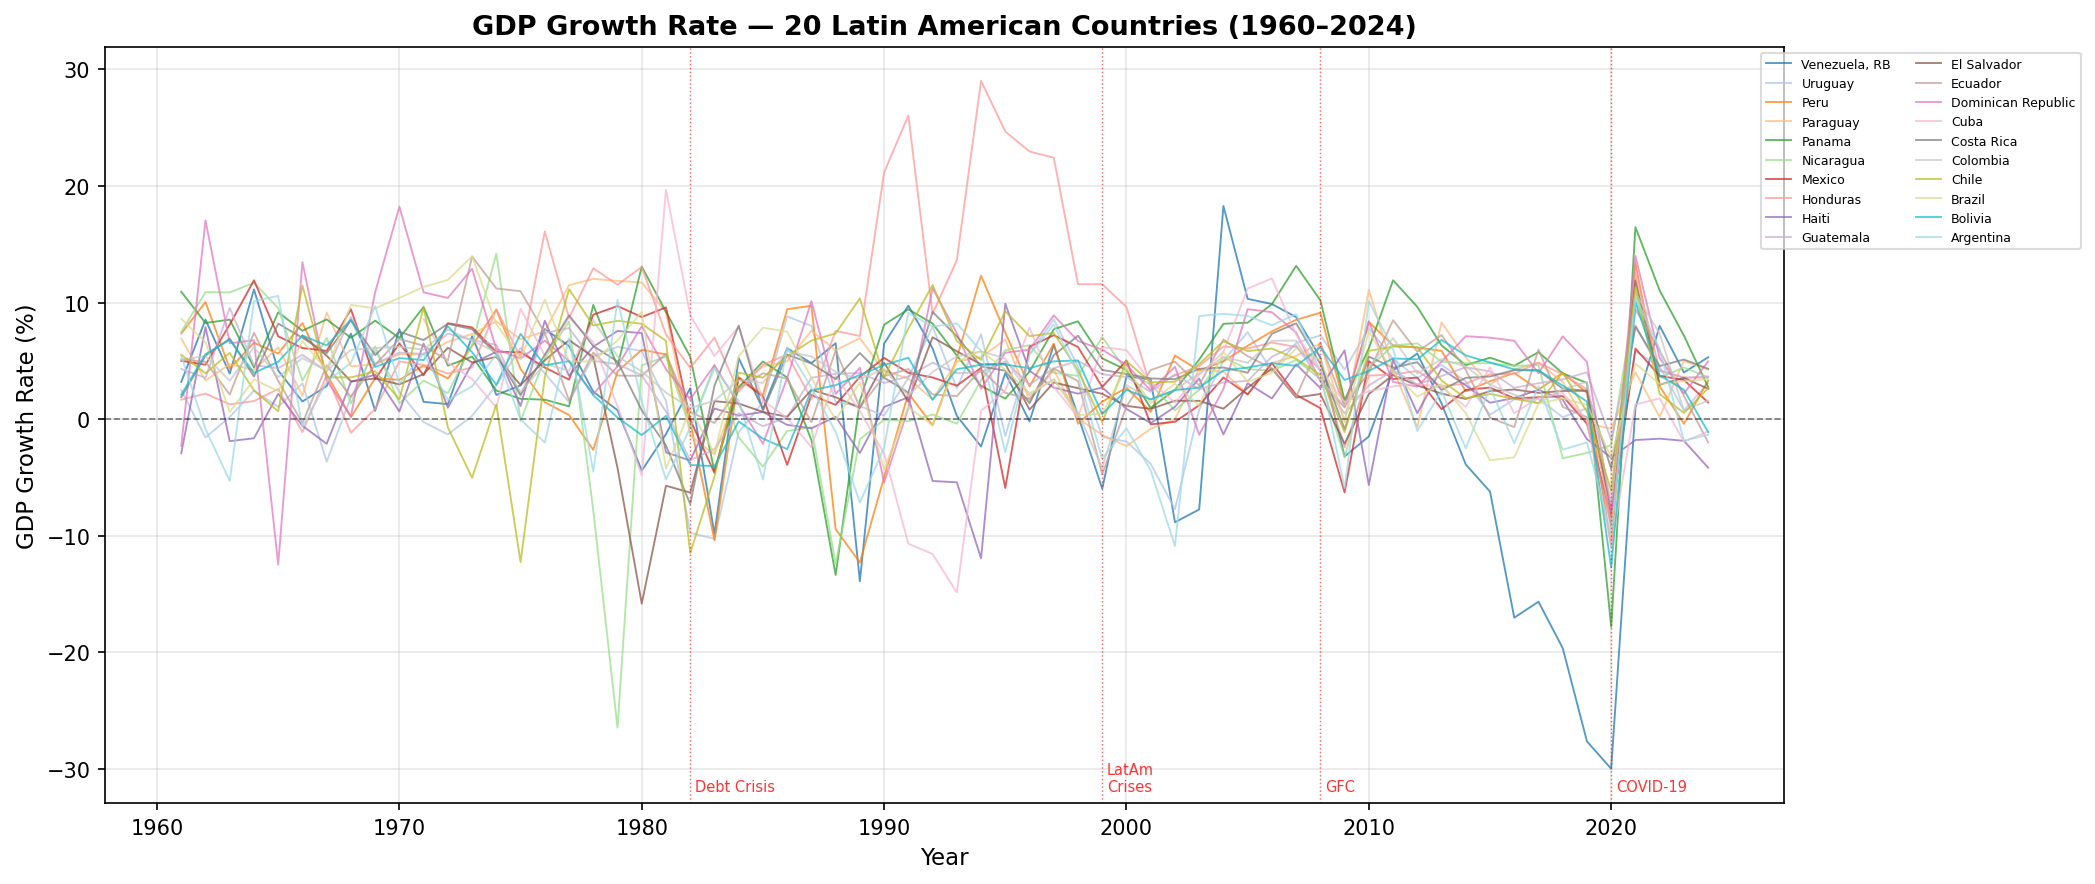
\includegraphics[width=\textwidth]{figures/fig01_all_trajectories.png}
  \caption{GDP growth rate trajectories for 20 Latin American countries,
           1960--2024. Red dotted lines mark major regional crises.}
  \label{fig:trajectories}
\end{figure}
Figure~\ref{fig:trajectories} presents the GDP growth trajectories for all 20
countries over the period 1960--2024. The data exhibits three defining
characteristics that motivate the methodological choices of this thesis.

First, the series is \emph{heteroskedastic}: the cross-sectional standard
deviation of growth rates varies substantially over time. 

\begin{figure}[H]
  \centering
  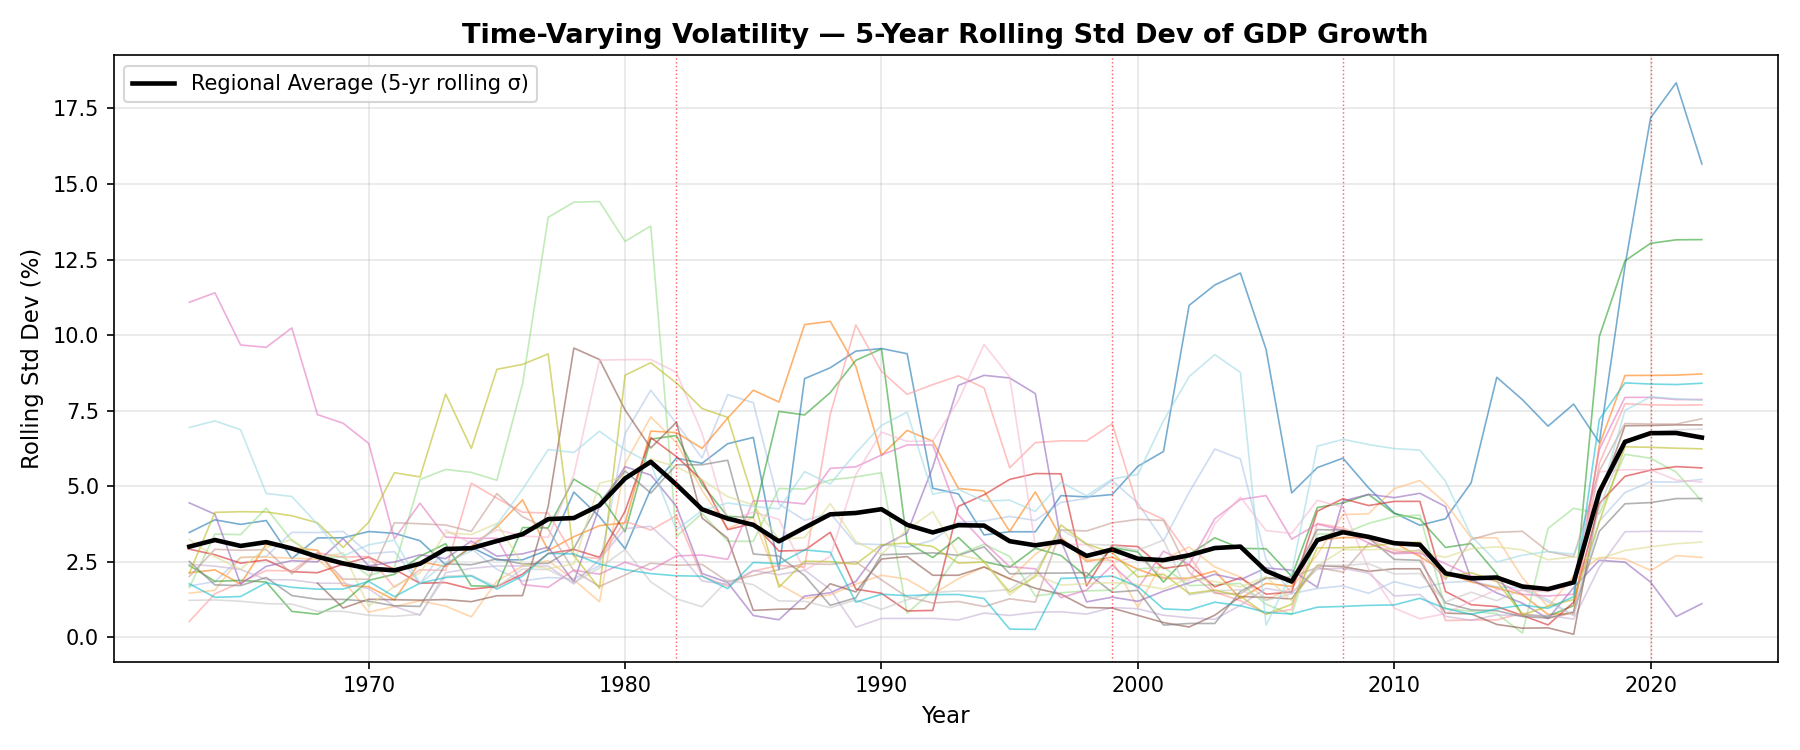
\includegraphics[width=\textwidth]{figures/fig06_rolling_volatility.png}
  \caption{Rolling std (time-varying volatility).}
  \label{fig:rolling_vol}
\end{figure}
Figure~\ref{fig:rolling_vol}
shows the 5-year rolling standard deviation, which peaks near the 1982 Latin
American Debt Crisis and again after the 2020 COVID-19 contraction, with a
relatively calm period from approximately 1995 to 2015. This non-stationarity
of variance violates the global smoothness assumptions underlying both B-spline
and Fourier bases.

Second, \emph{country-level volatility is highly heterogeneous}. Venezuela records
the highest standard deviation ($\hat{\sigma} = 8.76\%$), more than three times
that of Guatemala ($\hat{\sigma} = 2.40\%$), the most stable economy in the
sample (Figure~\ref{fig:vol_bars}). This heterogeneity implies that a single
smoothing parameterisation cannot be appropriate for all countries simultaneously.

Third, the GDP growth heatmap (Figure~\ref{fig:heatmap}) reveals that the major
regional crises---the 1982 Debt Crisis, the 1999 LatAm crises, the 2008 Global
Financial Crisis, and the 2020 COVID-19 contraction---affect countries with
different timing, magnitude, and duration. This \emph{temporal localisation} of
shocks is the key property motivating the wavelet basis: unlike Fourier methods,
which describe variation globally across the entire time domain, wavelets localise
simultaneously in time and frequency.


\begin{figure}[H]
  \centering
  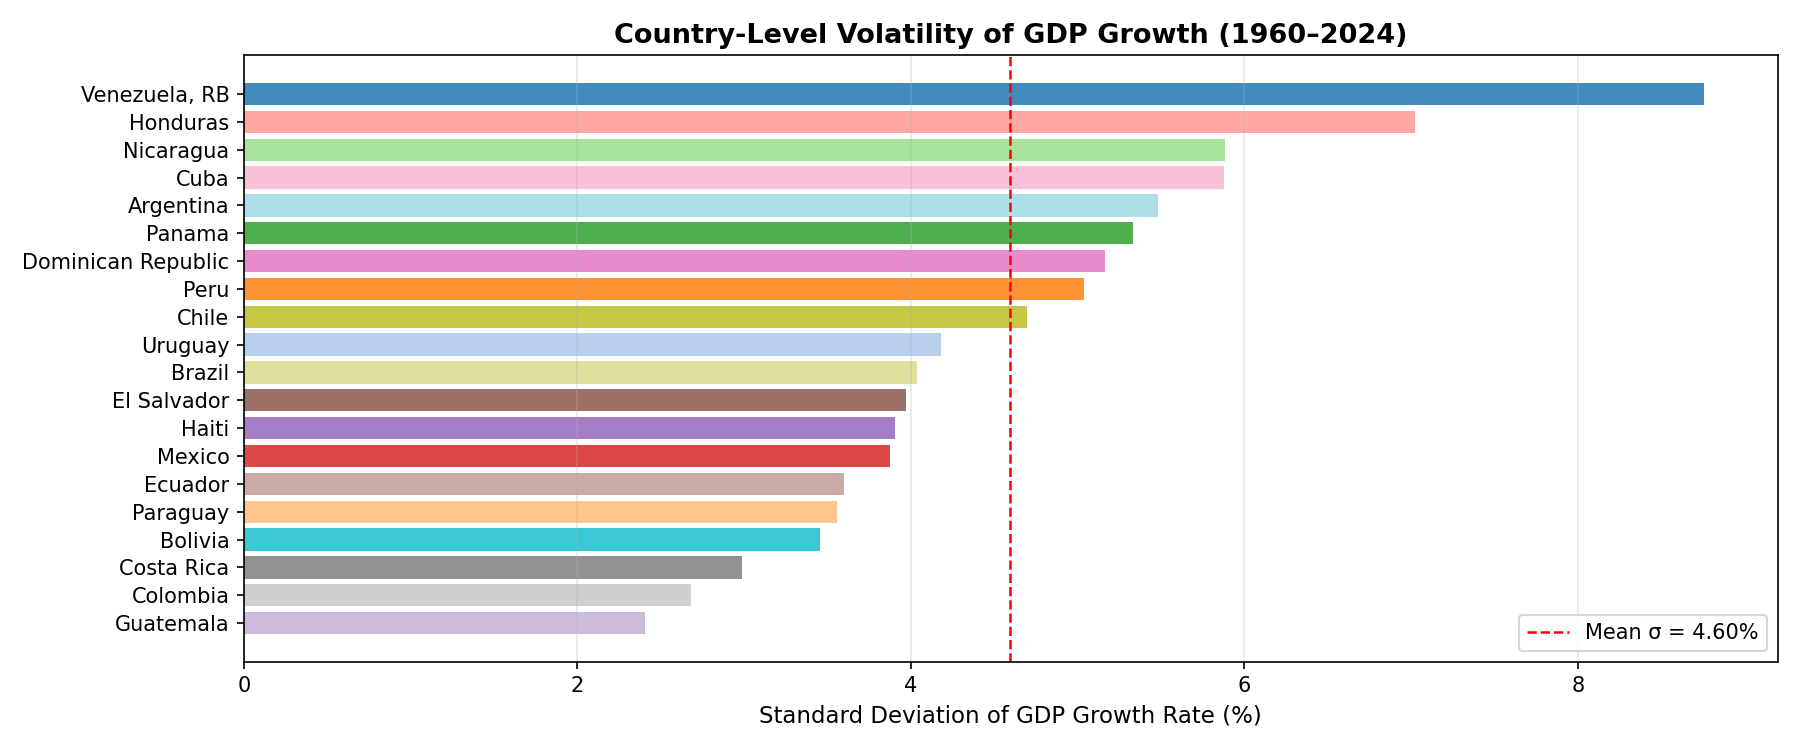
\includegraphics[width=\textwidth]{figures/fig03_volatility_bars.png}
  \caption{Country volatility bar chart}
  \label{fig:vol_bars}
\end{figure}

\begin{figure}[H]
  \centering
  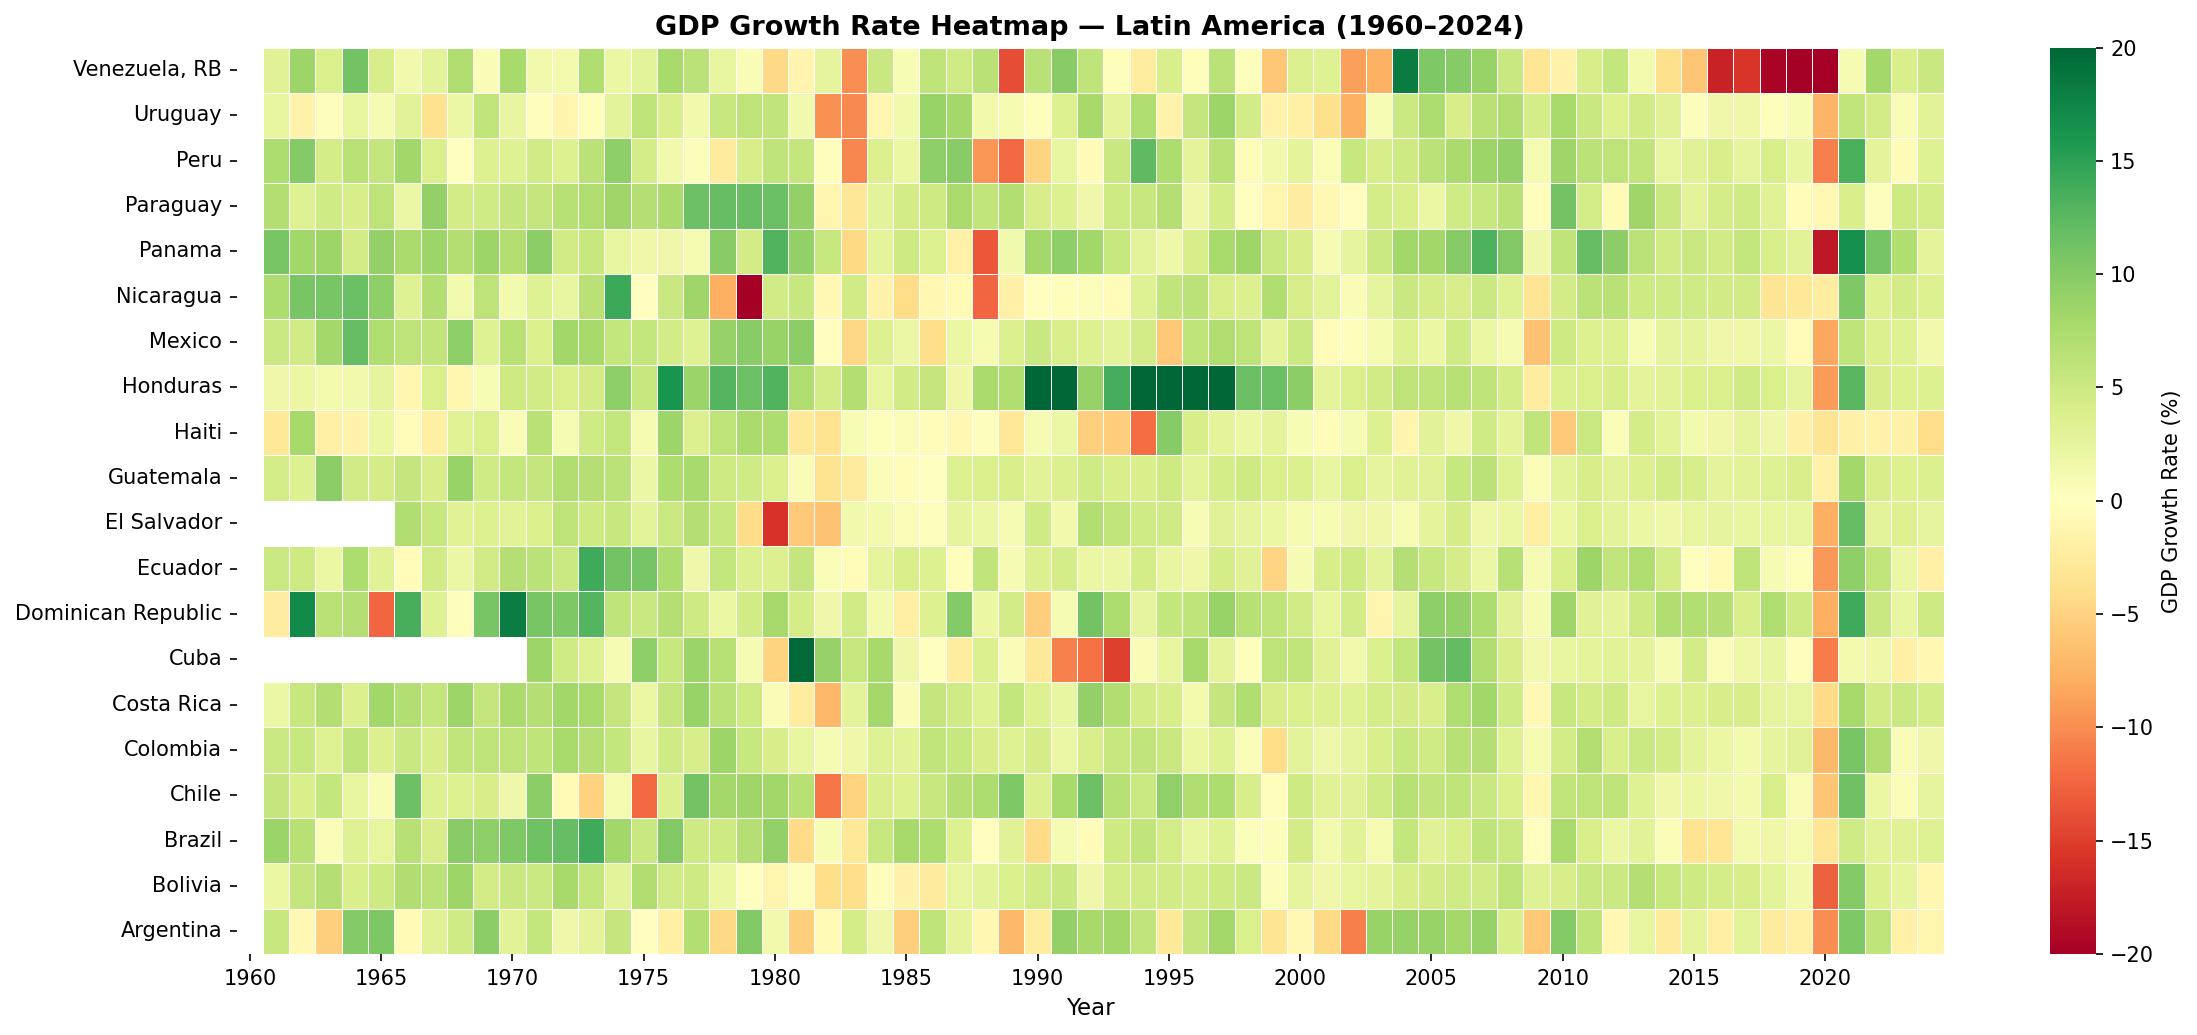
\includegraphics[width=\textwidth]{figures/fig04_heatmap.png}
  \caption{Heatmap of GDP growth over time}
  \label{fig:heatmap}
\end{figure}


\section{Basis Expansion Results}
\label{sec:basis_results}

\subsection{Reconstruction Quality and Coefficient Economy}
\label{subsec:coeff_economy}

Table~\ref{tab:rmse_summary} reports the mean RMSE across all 20 countries for
each basis configuration at matched smoothing levels. As explained in
Section~\ref{subsec:rmse}, wavelets are evaluated at the per-country threshold
$\lambda^*$ that matches the B-spline RMSE, so that the comparison is made at
equivalent reconstruction quality.

\begin{table}[H]
\centering
\caption{Mean RMSE and coefficient use across all 20 countries. Wavelet columns
report results at the threshold $\lambda^*$ matched to the B-spline RMSE of each
country individually.}
\label{tab:rmse_summary}
\begin{tabular}{lrrr}
\hline
\textbf{Method} & \textbf{Mean RMSE} & \textbf{Mean coeff.\ used} & \textbf{Total coeff.} \\
\hline
B-spline (adaptive)        & 2.51 & 19.5 knots & --- \\
Fourier ($K = 15$)         & 2.65 & 29         & 65  \\
Wavelet DB2  ($\lambda^*$) & 2.52 & 38.8       & 128 \\
Wavelet Sym4 ($\lambda^*$) & 2.53 & 38.0       & 128 \\
\hline
\end{tabular}
\end{table}

\begin{figure}[H]
  \centering
  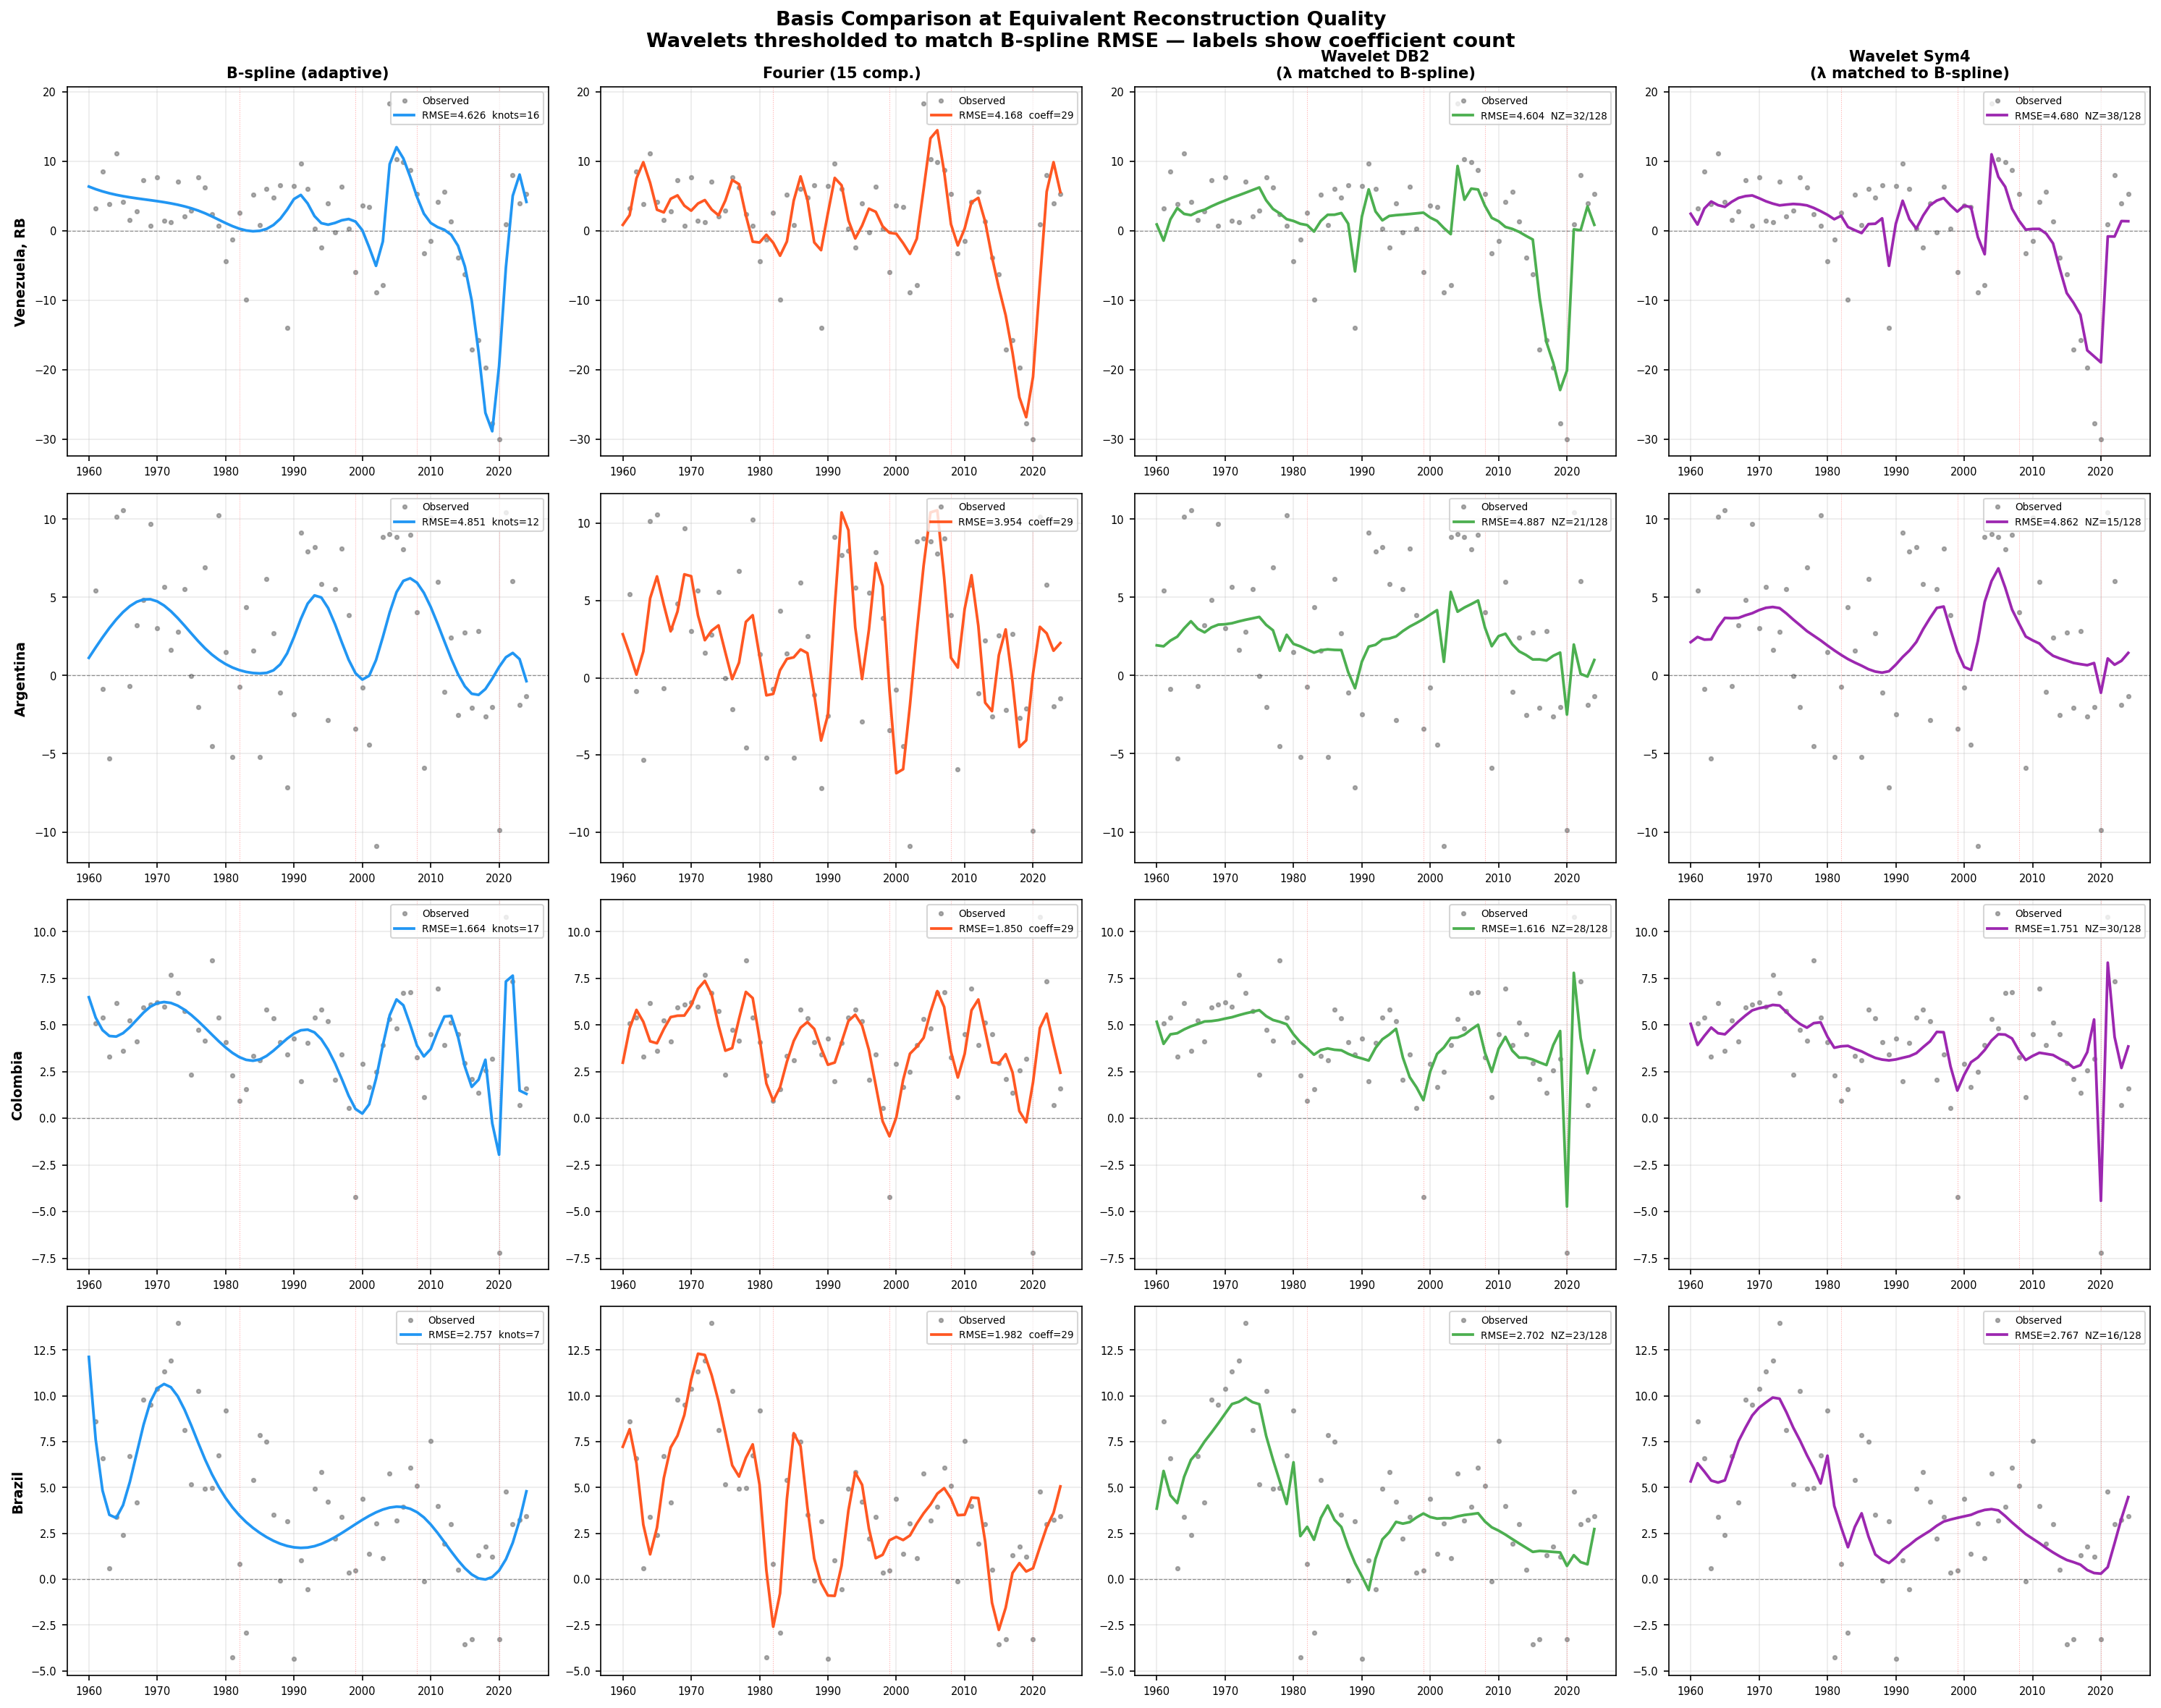
\includegraphics[width=\textwidth]{figures/fig07b_fair_comparison.png}
  \caption{Basis comparison grid.}
  \label{fig:fair_comparison}
\end{figure}

The B-spline achieves the lowest mean RMSE with the fewest knots (19.5 on
average). However, as Figure~\ref{fig:fair_comparison} demonstrates for
Venezuela, Argentina, Colombia, and Brazil, this apparent parsimony is
misleading: the B-spline reconstruction completely suppresses the crisis
episodes that define the economic histories of the most volatile countries.
The smooth trend it recovers discards signal rather than compressing it.

At matched RMSE, the Sym4 wavelet requires on average 38 nonzero coefficients
out of a total of 128 (70\% compression), compared to the B-spline's 19.5 knots.
These 38 coefficients, however, preserve the crisis episodes. The remaining 90
zeroed coefficients correspond to genuinely small detail components whose
omission causes no perceptible distortion of the economic signal.

Figure~\ref{fig:coeff_economy} presents the coefficient count comparison for all
20 countries. The wavelet coefficient count correlates strongly with country
volatility: Venezuela, Honduras, and Nicaragua---the three most volatile
economies---require the most nonzero wavelet coefficients to match B-spline
smoothing quality. This is direct empirical confirmation that their GDP
trajectories are less regular in the Besov sense.

\begin{figure}[H]
  \centering
  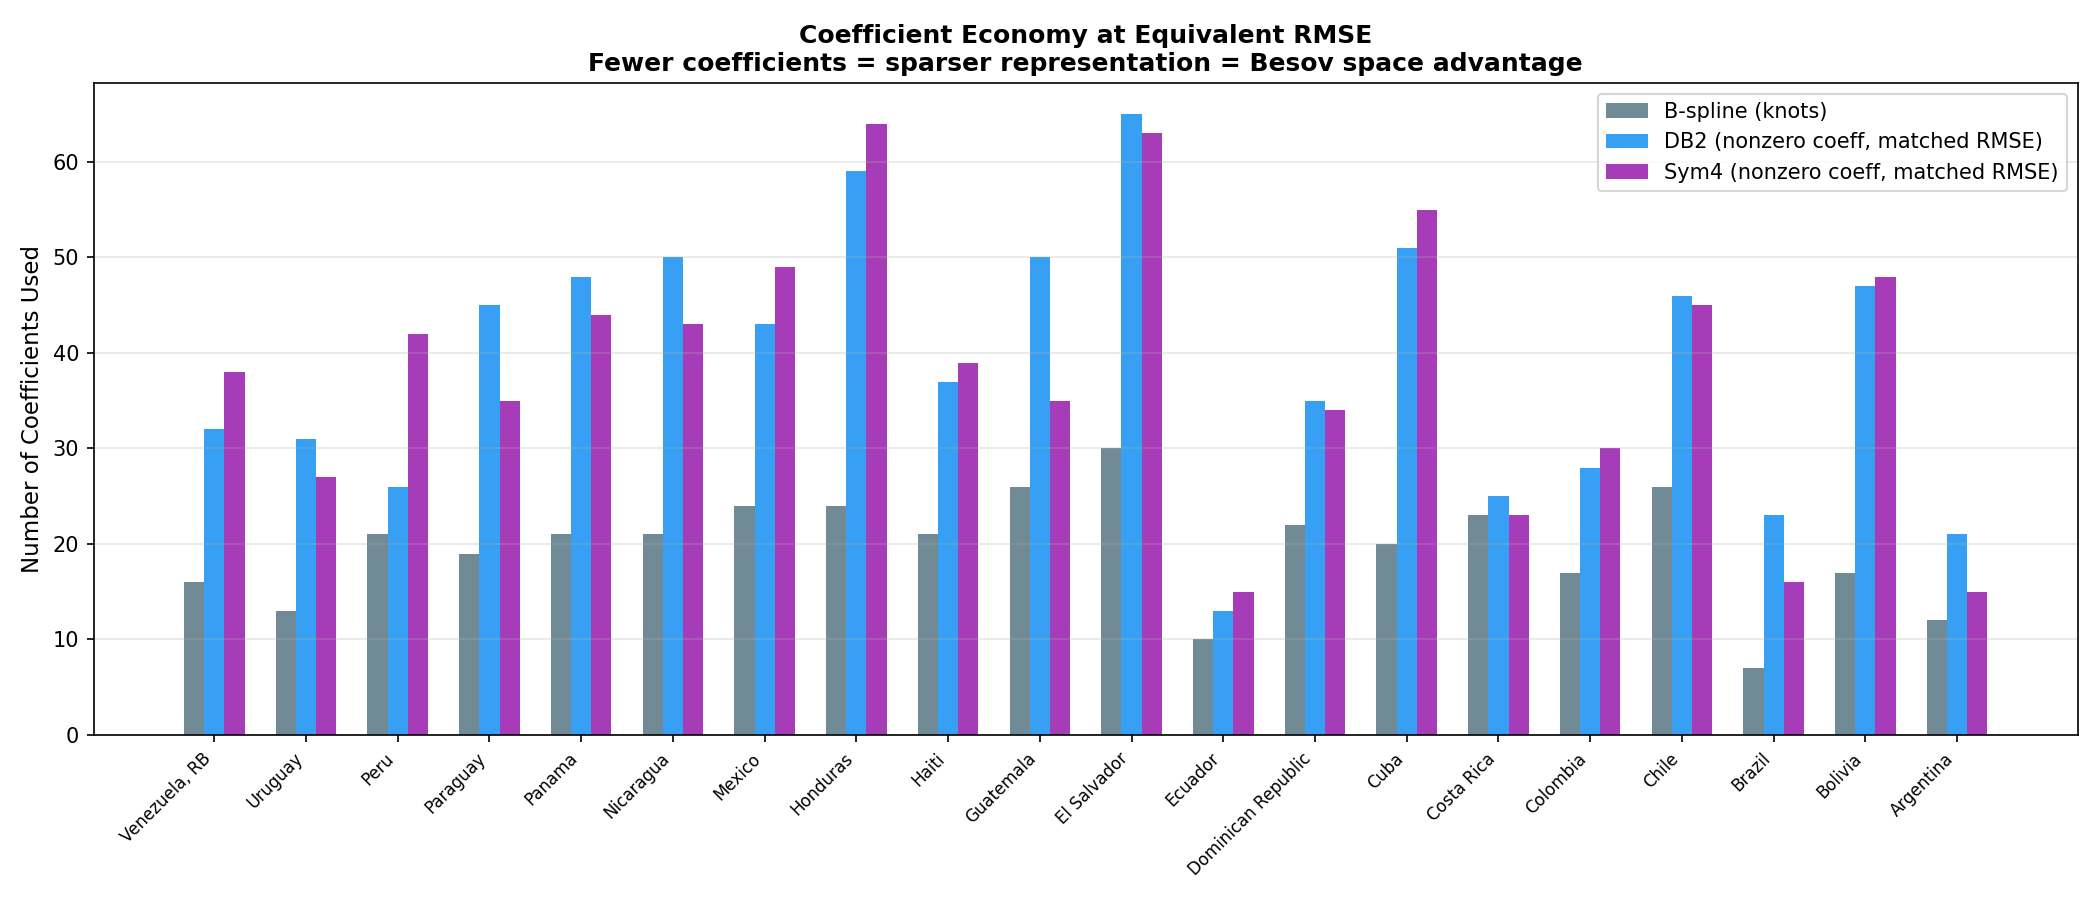
\includegraphics[width=\textwidth]{figures/fig12_coefficient_economy.png}
  \caption{RMSE vs sparsity curves.}
  \label{fig:coeff_economy}
\end{figure}

\begin{figure}[H]
  \centering
  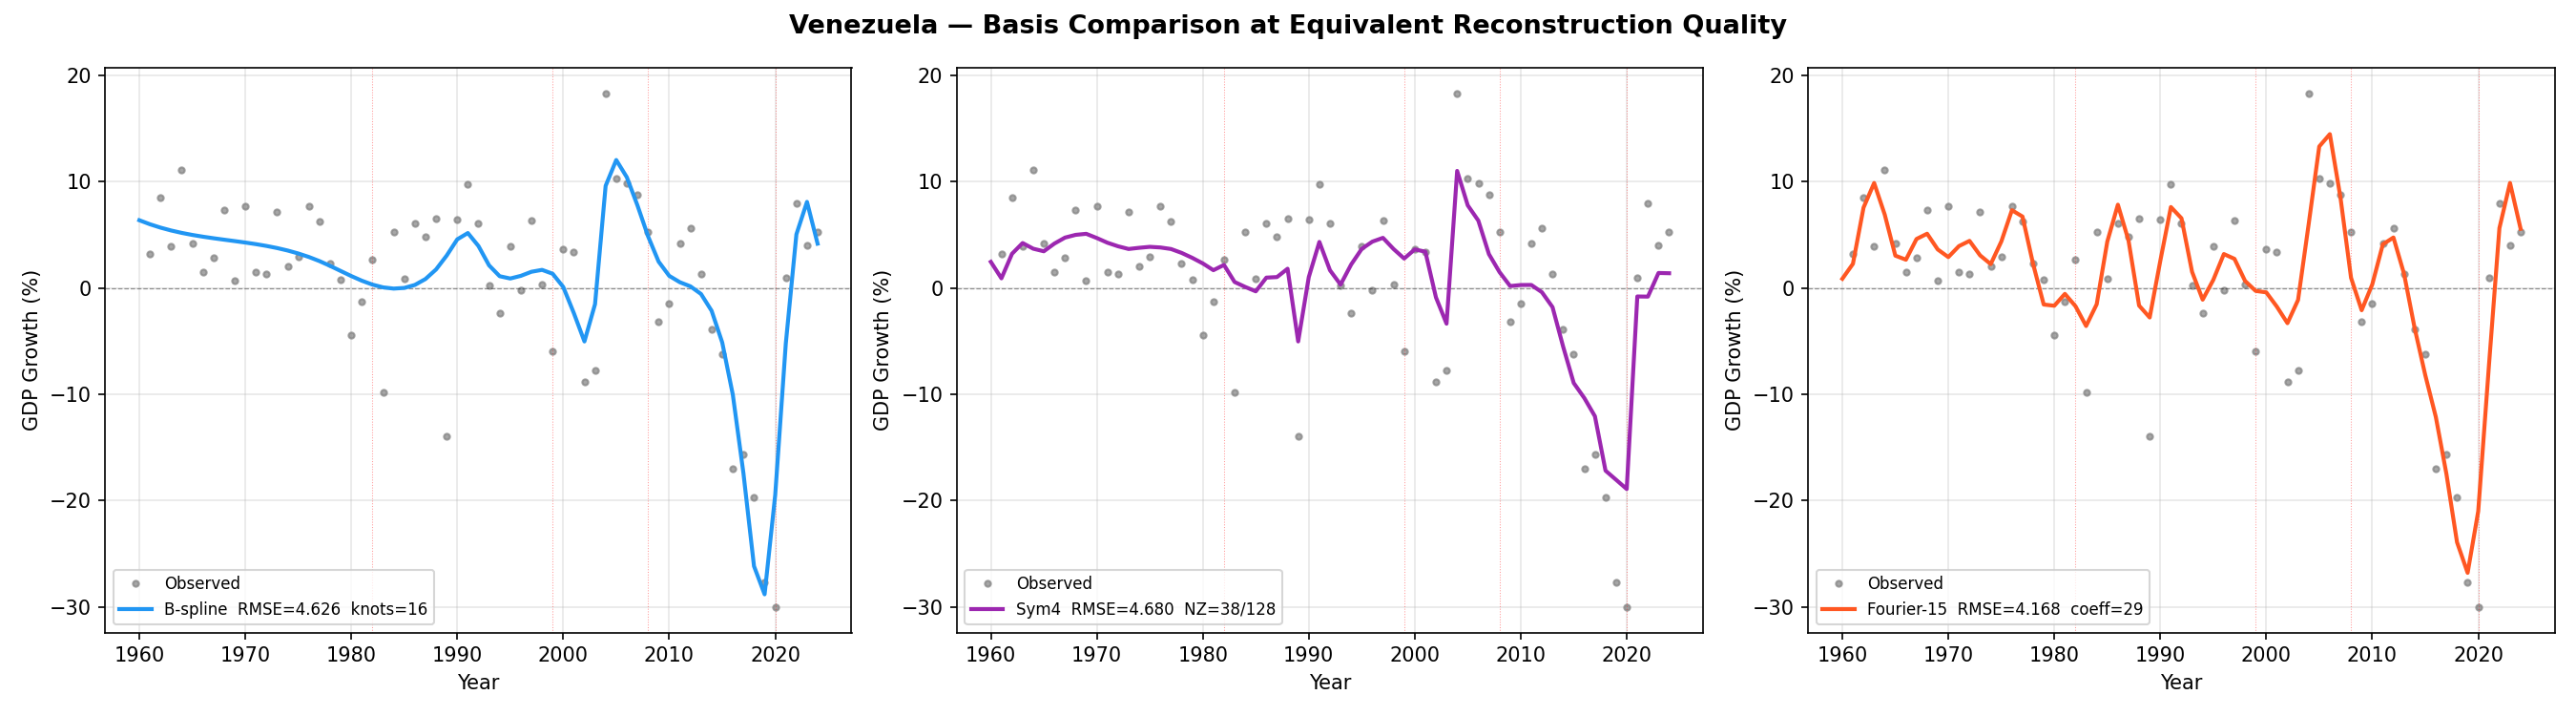
\includegraphics[width=\textwidth]{figures/fig14_venezuela_comparison.png}
  \caption{Venezuela: B-spline vs Sym4 at matched RMSE side by side.}
  \label{fig:venezuela_comparison}
\end{figure}

The Venezuela case (Figure~\ref{fig:venezuela_comparison}) illustrates the
qualitative differences most sharply. The B-spline (RMSE = 4.63, 16 knots)
produces a monotone declining trend from 2000 onward that misses both the
2004--2008 oil boom and the catastrophic 2015--2020 contraction. The Sym4 wavelet
at matched RMSE (38/128 nonzero coefficients) correctly identifies both episodes
while remaining appropriately smooth during the stable 1960--1990 period. The
Fourier reconstruction (15 components, RMSE = 4.17) introduces visible spurious
oscillations during the stable 1960--1990 period, consistent with the Gibbs
phenomenon discussed in Section~\ref{subsec:gibbs_results} below.

\subsection{Sparsity-Fidelity Tradeoff and the Besov Space Argument}
\label{subsec:sparsity_results}

\begin{figure}[H]
  \centering
  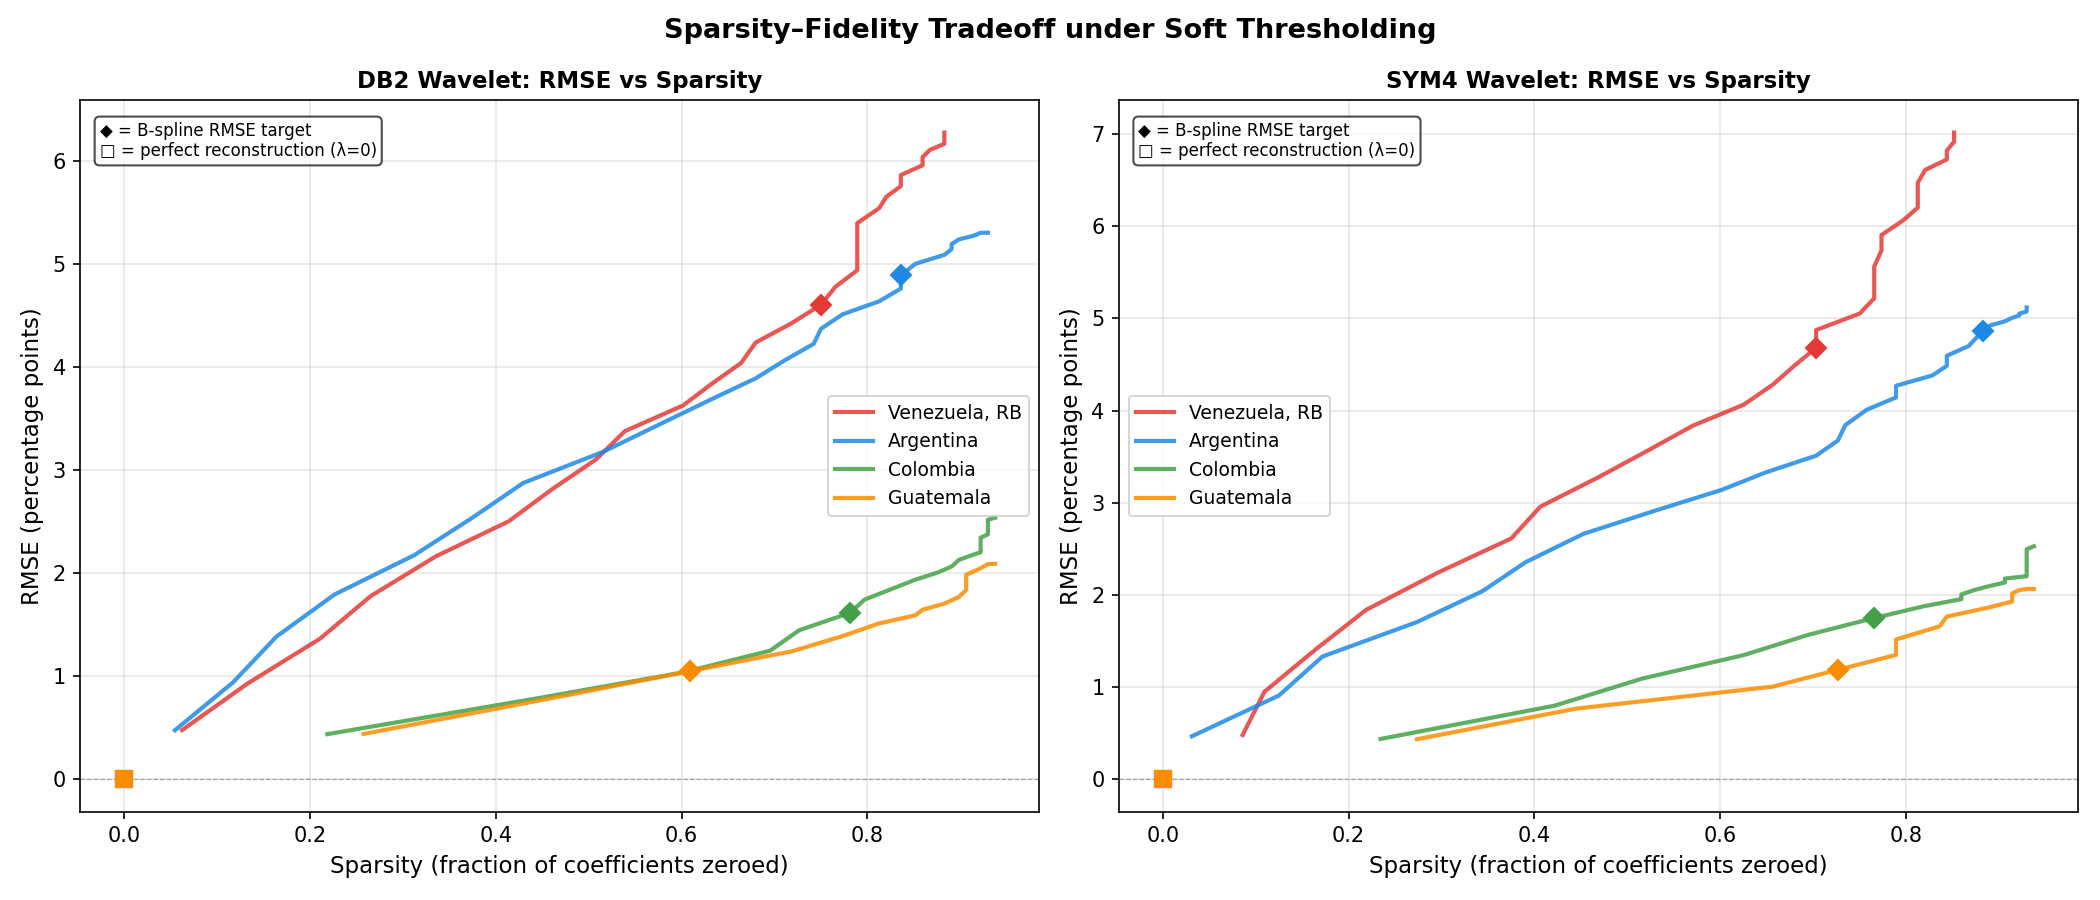
\includegraphics[width=\textwidth]{figures/fig13_sparsity_fidelity.png}
  \caption{Wavelet energy distribution.}
  \label{fig:sparsity_tradeoff}
\end{figure}

Figure~\ref{fig:sparsity_tradeoff} presents the sparsity-fidelity tradeoff
curves for four countries of contrasting volatility under Sym4 and DB2 wavelet
thresholding. Each curve traces RMSE as a function of the fraction of
coefficients zeroed as $\lambda$ increases from 0 to 15.

The shape of these curves provides direct empirical evidence for the Besov space
characterisation. For Guatemala and Colombia---the two least volatile economies
in the sample---the curves are relatively flat: RMSE increases slowly as
coefficients are zeroed, meaning the GDP trajectories of these countries are
genuinely sparse in the wavelet basis and live near a Besov ball of high
regularity. For Venezuela and Argentina, the curves are steep: significant RMSE
accumulates rapidly as coefficients are zeroed, consistent with lower Besov
regularity arising from the multiscale shocks that characterise these economies.

This country-specific regularity structure is invisible to B-splines or Fourier
bases, which apply a single global smoothness criterion to all countries. The
wavelet basis, by contrast, adapts to the local regularity of each trajectory,
providing a richer characterisation of cross-country heterogeneity in economic
volatility. The marked diamond on each curve in Figure~\ref{fig:sparsity_tradeoff}
indicates the B-spline RMSE target: stable economies reach this target at higher
sparsity levels (more efficient compression), while volatile economies reach it
at lower sparsity levels.



\subsection{Fourier Basis and the Gibbs Phenomenon}
\label{subsec:gibbs_results}

The power spectrum of Venezuelan GDP growth (Figure~\ref{fig:fourier_spectrum})
shows no dominant peak at any specific period. Power is broadly distributed
across 15--35 year periods, inconsistent with a regular business cycle and
suggesting that the growth process is driven by aperiodic commodity and political
shocks rather than a deterministic cycle. This undermines the theoretical
motivation for the Fourier basis on this dataset.


\begin{figure}[H]
  \centering
  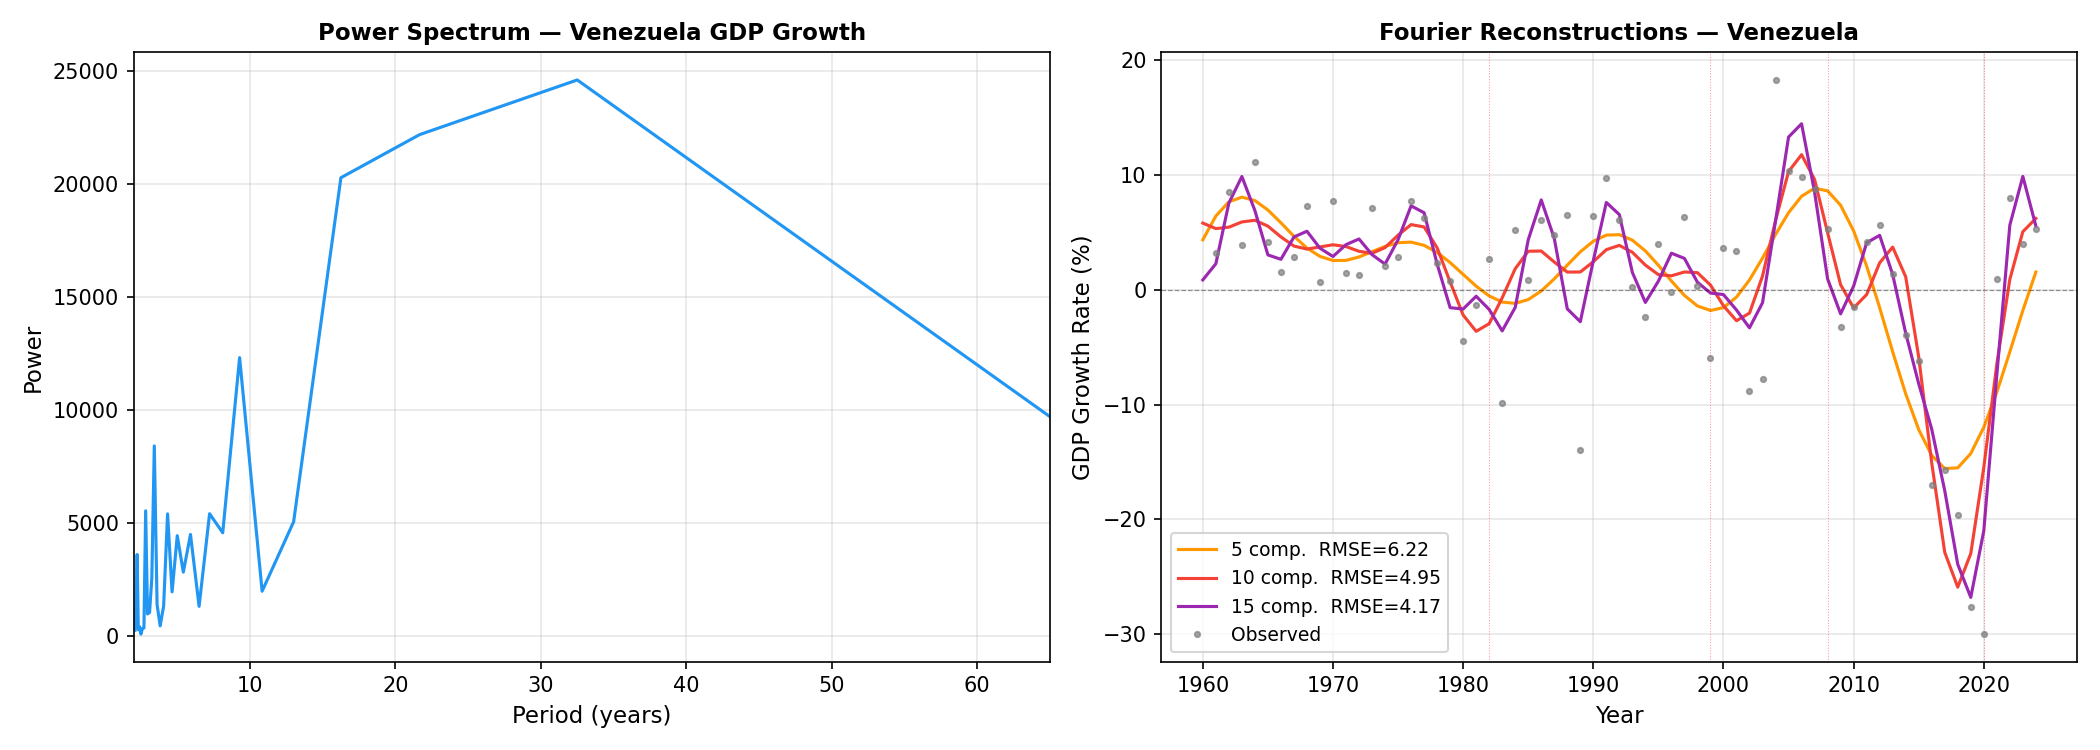
\includegraphics[width=\textwidth]{figures/fig10_fourier_spectrum_venezuela.png}
  \caption{Fourier spectrum — Venezuela.}
  \label{fig:fourier_spectrum}
\end{figure}


Empirically, increasing the number of Fourier components from 5 to 15 reduces
RMSE from 6.22 to 4.17 for Venezuela, but introduces visible spurious oscillations
during the stable 1960--1995 period (Figure~\ref{fig:venezuela_comparison},
right panel). This is consistent with the Gibbs phenomenon: the finite-term
Fourier approximation oscillates near the structural breaks at 1983 and 2020,
corrupting the representation of surrounding smooth periods. Fourier-15 requires
29 coefficients to achieve mean RMSE = 2.65 across all countries, comparable to
B-splines, but at the cost of these Gibbs-type artefacts near crisis years.

\section{FPCA Results}
\label{sec:fpca_results}

\subsection{Replication of the Original Result}
\label{subsec:replication}

Table~\ref{tab:fpca_summary} extends Table~2 of \cite{padilla2020} to include
all basis configurations tested in this thesis.

\begin{table}[H]
\centering
\caption{FPCA variance explanation results. $\mathrm{VE}_k$ denotes the percentage
of variance explained by the $k$-th FPC; $n_{80}$ is the number of FPCs required
to explain at least 80\% of total variance. The original paper result is included
for direct comparison.}
\label{tab:fpca_summary}
\begin{tabular}{lrrrrr}
\hline
\textbf{Configuration} & $\mathrm{\mathbf{VE_1}}$ & $\mathrm{\mathbf{VE_2}}$
    & $\mathrm{\mathbf{VE_3}}$ & \textbf{3-FPC} & $\mathbf{n_{80}}$ \\
\hline
Raw data (baseline)                    & 21.3\% & 15.9\% & 10.0\% & 47.2\% & 8 \\
B-spline (smooth $\sigma\!\times\!2$)  & 53.5\% & 25.0\% & 10.8\% & 89.2\% & 3 \\
Fourier ($K = 5$)                      & 40.4\% & 22.5\% & 12.5\% & 75.4\% & 4 \\
Fourier ($K = 15$)                     & 26.9\% & 17.6\% & 11.4\% & 55.9\% & 7 \\
Wavelet Sym4 ($\lambda = 0$, lossless) & 21.3\% & 15.9\% & 10.0\% & 47.2\% & 8 \\
Wavelet Sym4 ($\lambda = 5$)           & 33.8\% & 22.9\% & 10.8\% & 67.6\% & 5 \\
Wavelet Sym4 ($\lambda = 12$)          & 45.8\% & 27.0\% & 13.4\% & 86.2\% & 3 \\
Wavelet DB2  ($\lambda = 5$)           & 34.2\% & 23.6\% & 11.4\% & 69.1\% & 5 \\
Wavelet Haar ($\lambda = 5$)           & 32.6\% & 23.2\% & 11.3\% & 67.2\% & 5 \\
\hline
\multicolumn{6}{l}{\textit{Original paper \cite{padilla2020}:}} \\
B-spline order 5, dim 48               & 17.7\% & 16.5\% & 12.9\% & 47.1\% & $>8$ \\
\hline
\end{tabular}
\end{table}

The raw data FPCA (equivalent to an interpolating B-spline, $\lambda = 0$)
yields $\mathrm{VE_1} = 21.3\%$, $\mathrm{VE_2} = 15.9\%$,
$\mathrm{VE_3} = 10.0\%$, with a 3-FPC total of 47.2\%---nearly identical to
the original paper's 47.1\%. This confirms that the extended dataset (1960--2024
vs.\ 1970--2018) and revised country coverage preserve the essential variance
structure identified by \cite{padilla2020}, and validates the full pipeline
before proceeding to the alternative bases.

\subsection{Effect of Basis Choice on FPCA Parsimony}
\label{subsec:fpca_parsimony}

The cumulative variance curves in Figure~\ref{fig:cumvar} reveal a clear and
interpretable ordering among all configurations. The basis choice has a dramatic
effect on FPCA parsimony, but this effect must be interpreted carefully rather
than equated with quality.

B-spline smoothing ($\sigma\!\times\!2$) requires only 3 FPCs for 80\% variance
explained. However, Figure~\ref{fig:fpc1_shapes} shows that the B-spline FPC1
is a monotone declining trend, capturing the post-1980 growth slowdown and
explaining 53.5\% of variance. This high parsimony arises because smoothing has
removed the crisis variation and left only the trend. It is a poorer description
of the data---information has been discarded rather than organised.

\begin{figure}[H]
  \centering
  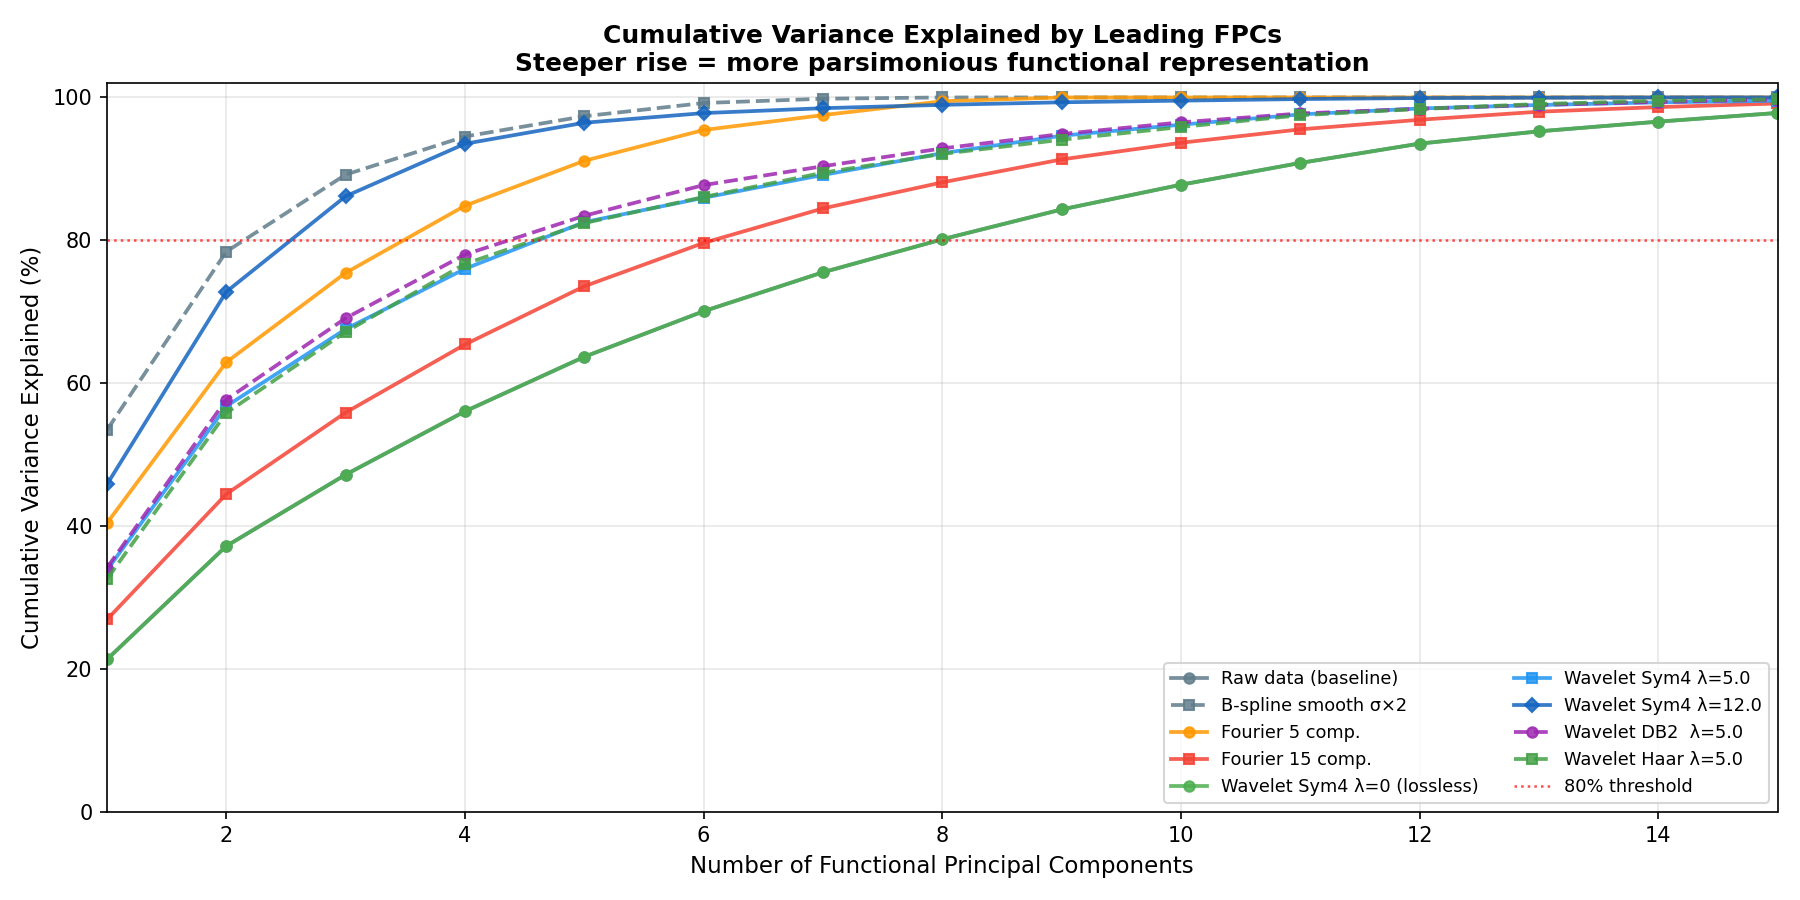
\includegraphics[width=\textwidth]{figures/fig18_cumvar_curves.png}
  \caption{Cumulative variance curves.}
  \label{fig:cumvar}
\end{figure}

\begin{figure}[H]
  \centering
  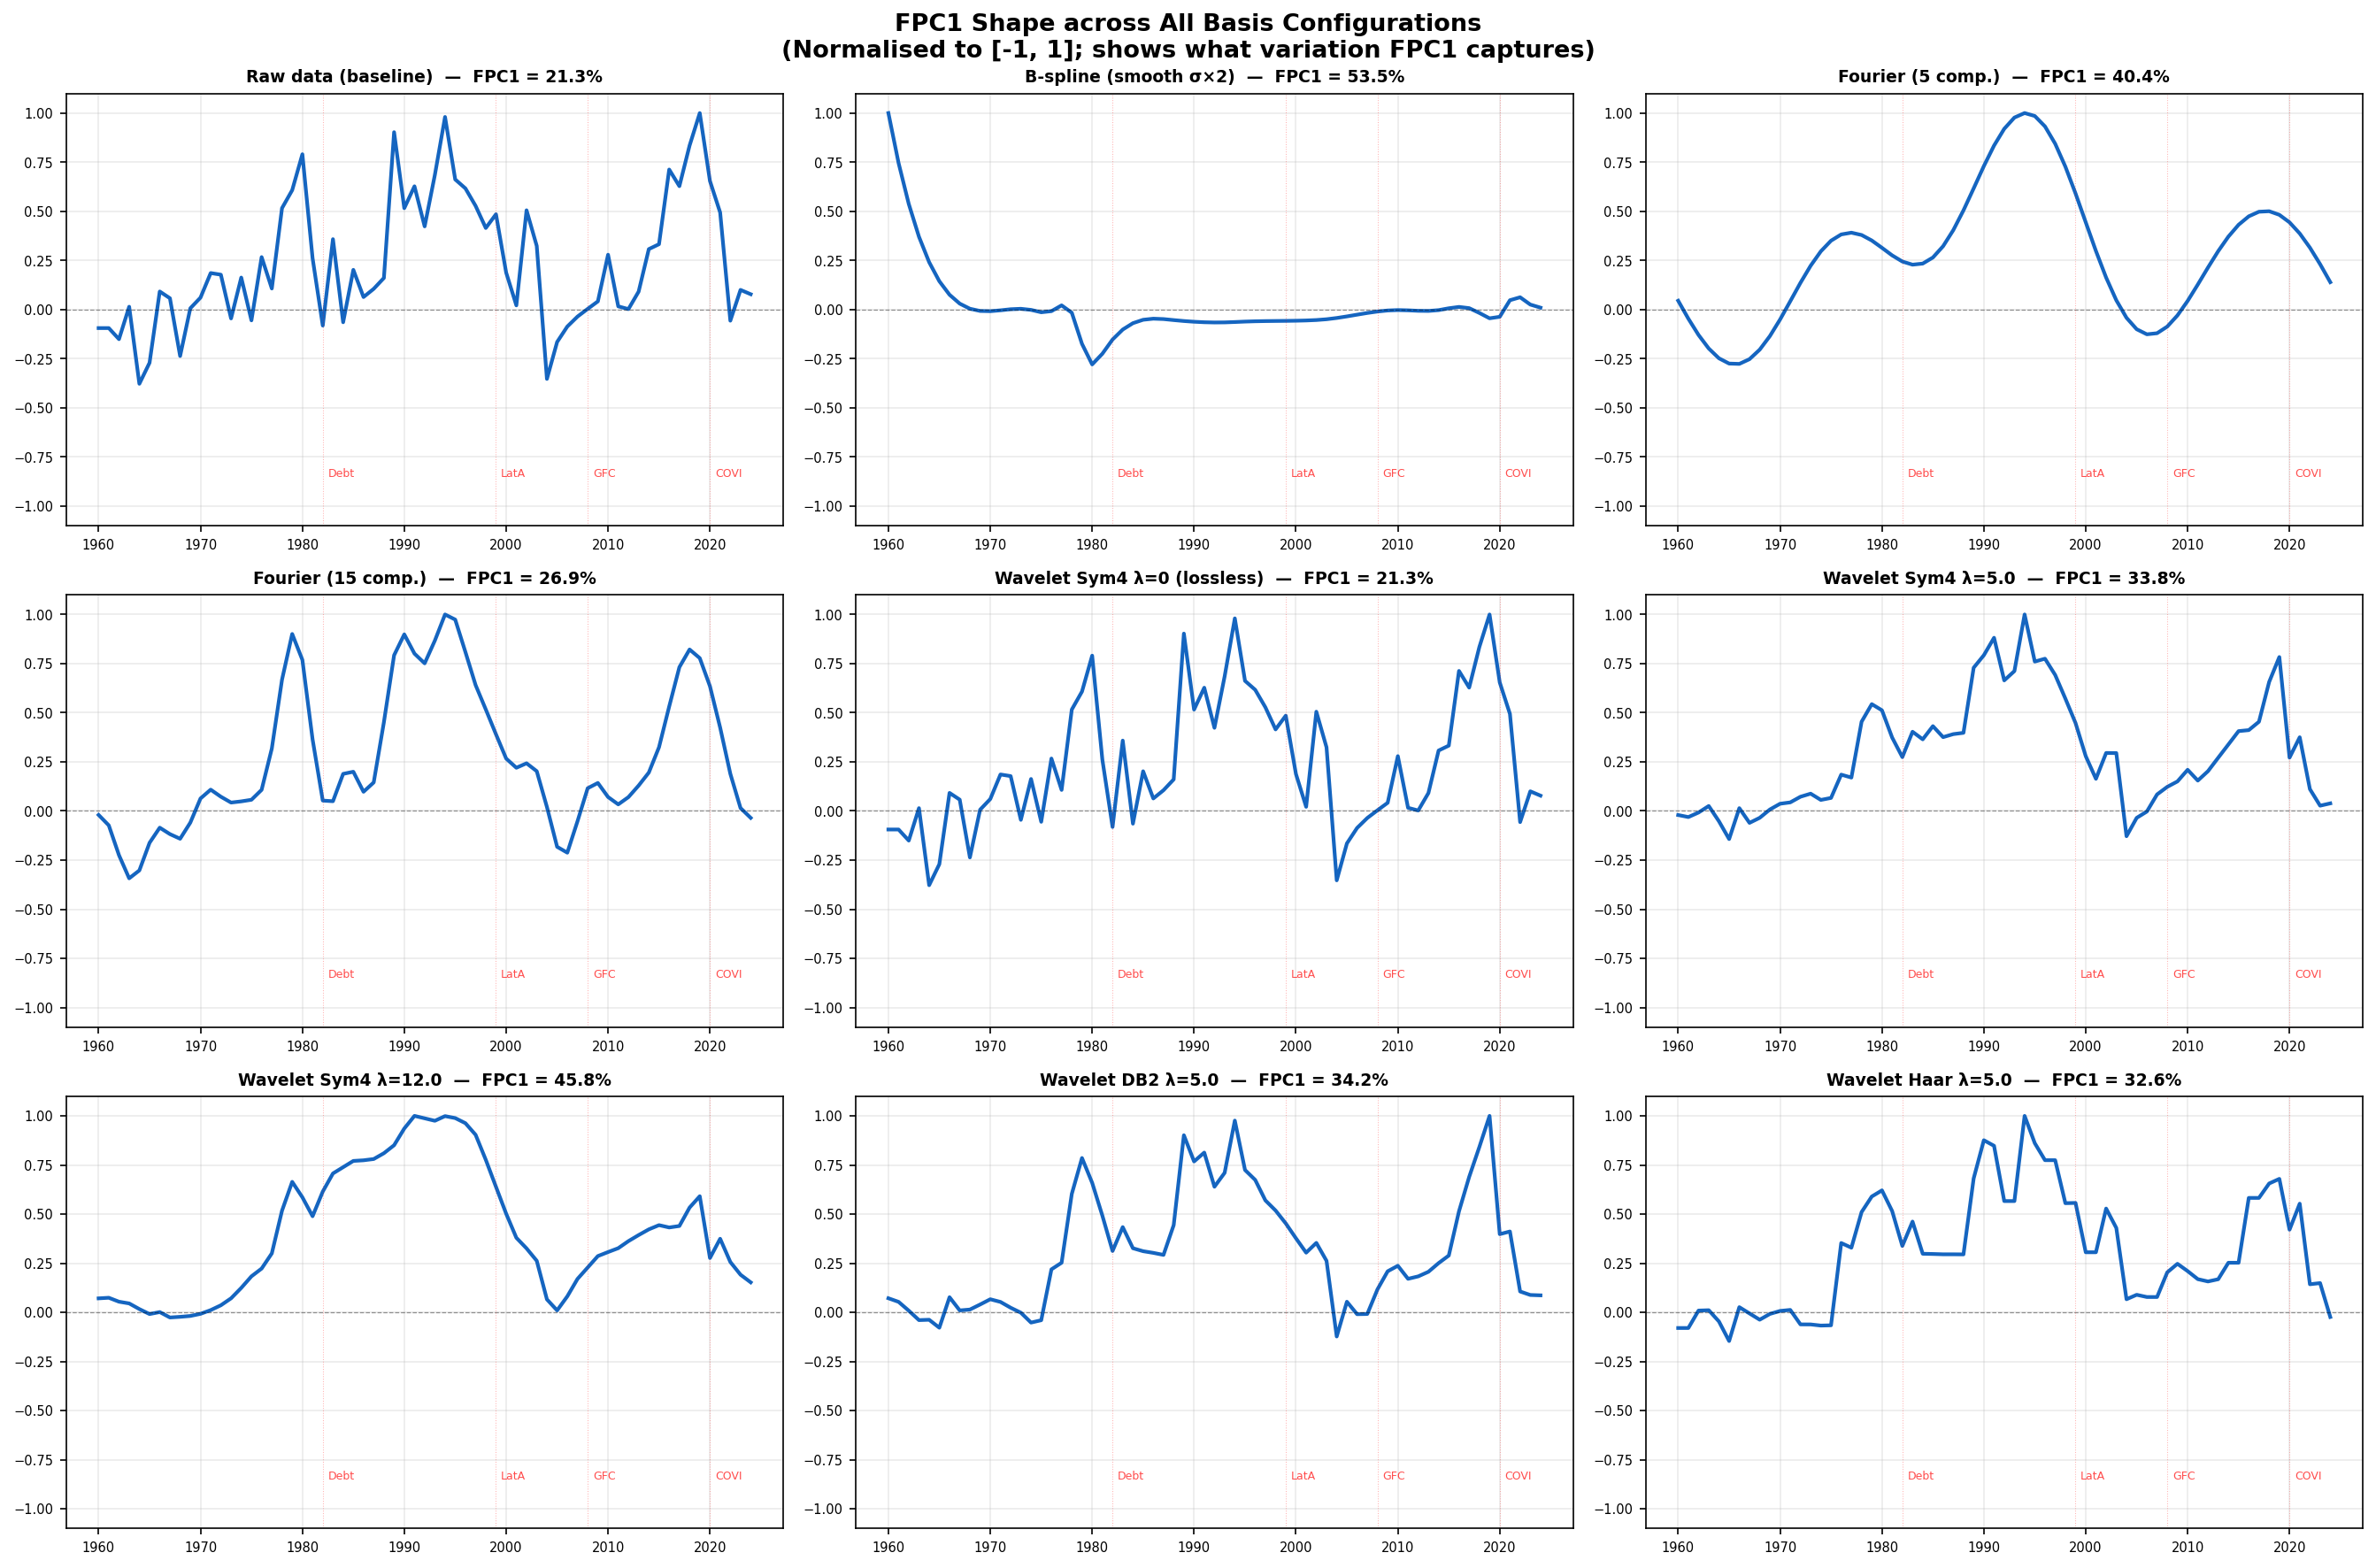
\includegraphics[width=\textwidth]{figures/fig19_fpc1_shapes.png}
  \caption{FPC1 curve comparison across bases.}
  \label{fig:fpc1_shapes}
\end{figure}

Wavelet Sym4 at $\lambda = 5$ achieves a qualitatively richer FPCA. FPC1
explains 33.8\% and, as visible in Figure~\ref{fig:fpc1_shapes}, shows a
structured pattern rising through the 1970s commodity boom, declining through
the 1982--1990 lost decade, recovering during the 2000s commodity super-cycle,
and collapsing sharply at COVID-19. This FPC1 is economically interpretable as
a \emph{commodity cycle} mode of variation---a regional factor driving correlated
growth fluctuations across commodity-exporting nations. Five FPCs are required
for 80\%, reflecting the genuine multidimensionality of cross-country variation
that the wavelet basis preserves rather than suppresses.

At $\lambda = 12$, the Sym4 wavelet converges toward the B-spline behaviour
($n_{80} = 3$), confirming that aggressive thresholding reduces the wavelet
representation to a smooth approximation. The threshold parameter $\lambda$
therefore acts as a \emph{continuous interpolation} between the raw data
representation ($\lambda = 0$, $n_{80} = 8$) and the smoothed representation
($\lambda \to \infty$, $n_{80} = 3$), giving the analyst direct control over
the parsimony-fidelity tradeoff. This interpolation property is visible as a
monotone family of curves in Figure~\ref{fig:cumvar}.

\subsection{FPC Mean Perturbation Plots}
\label{subsec:perturbation_plots}

\begin{figure}[H]
  \centering
  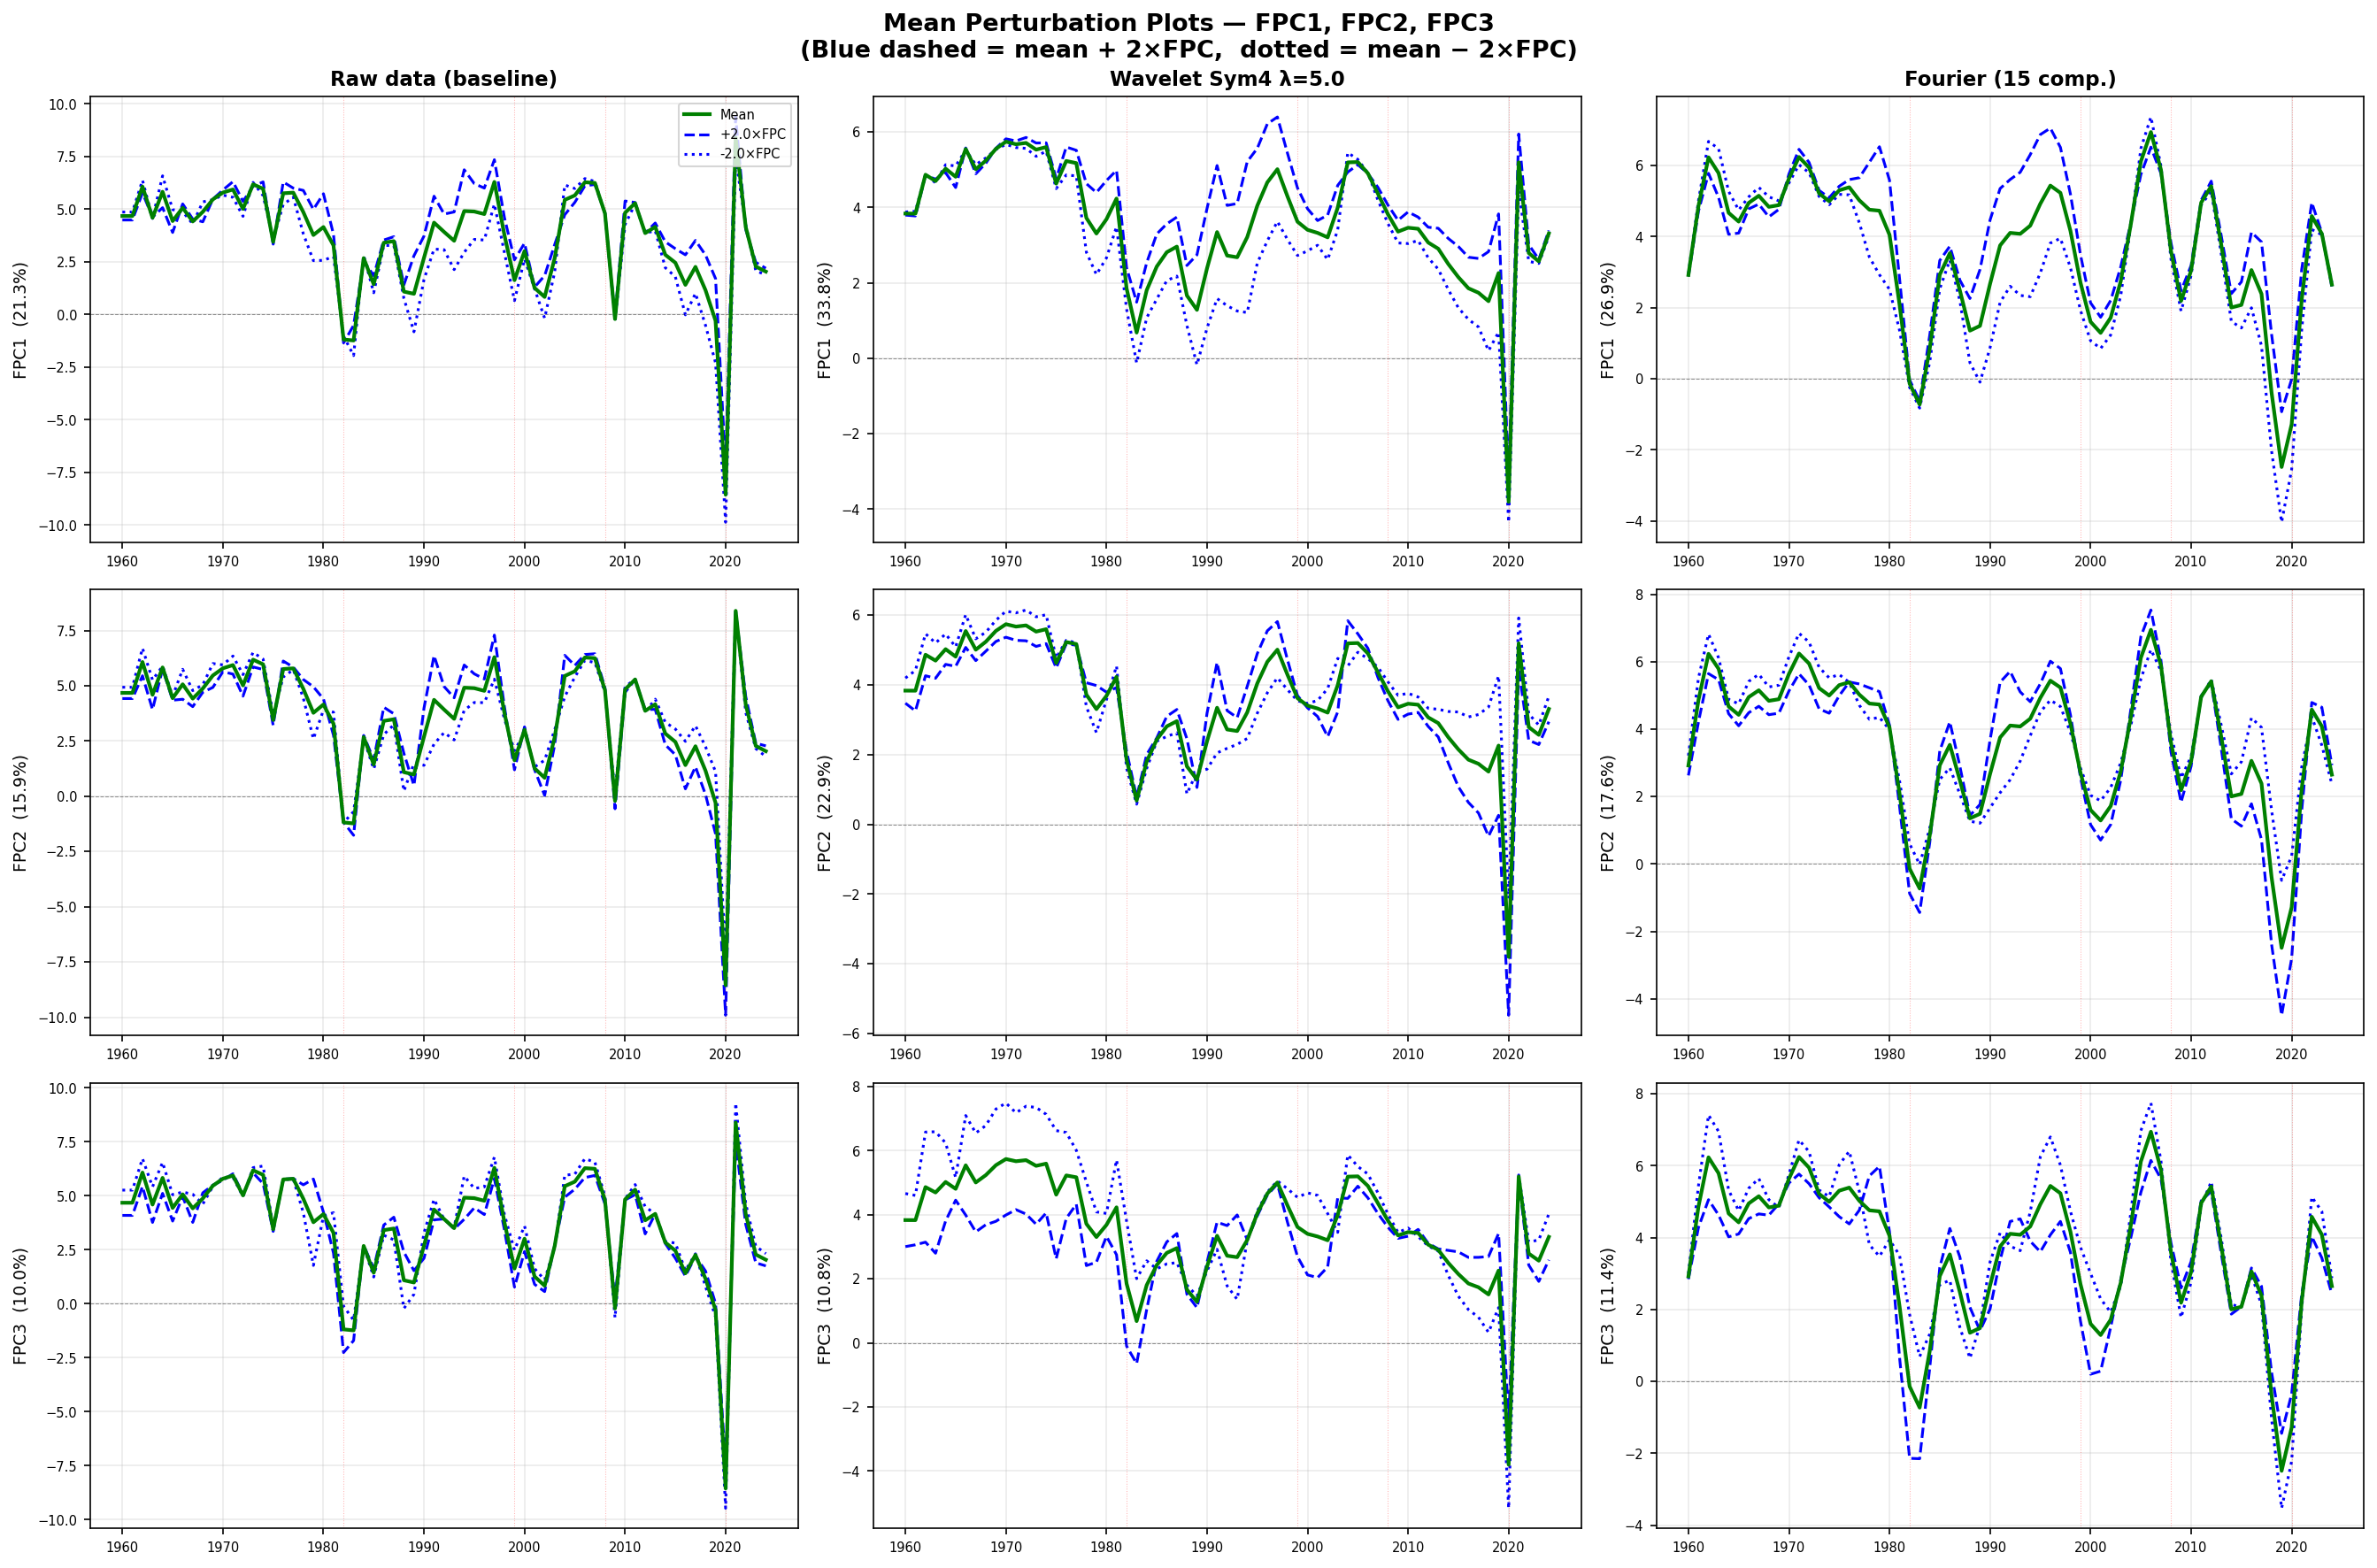
\includegraphics[width=\textwidth]{figures/fig16_fpc_perturbation_plots.png}
  \caption{FPC curves (perturbation plots).}
  \label{fig:perturbation}
\end{figure}

Figure~\ref{fig:perturbation} presents the mean perturbation plots for the
first three FPCs under three configurations (raw data, Wavelet Sym4 $\lambda = 5$,
and Fourier $K = 15$), replicating the style of Figure~7 in \cite{padilla2020}.

Under the raw data and lossless wavelet representations, the FPC perturbations
are small relative to the mean function and noisy in character, consistent with
individual crisis events being absorbed into the leading components. Under
Wavelet Sym4 $\lambda = 5$, the FPC1 perturbation band is structured and
economically legible: a country with a large positive FPC1 score grows faster
during the commodity boom decades and suffers a sharper post-2014 decline.
FPC2 under this representation captures a late-period divergence, separating
countries that recovered strongly after 2020 from those that did not.

\subsection{Score Plots and Country Separability}
\label{subsec:score_plots}

\begin{figure}[H]
  \centering
  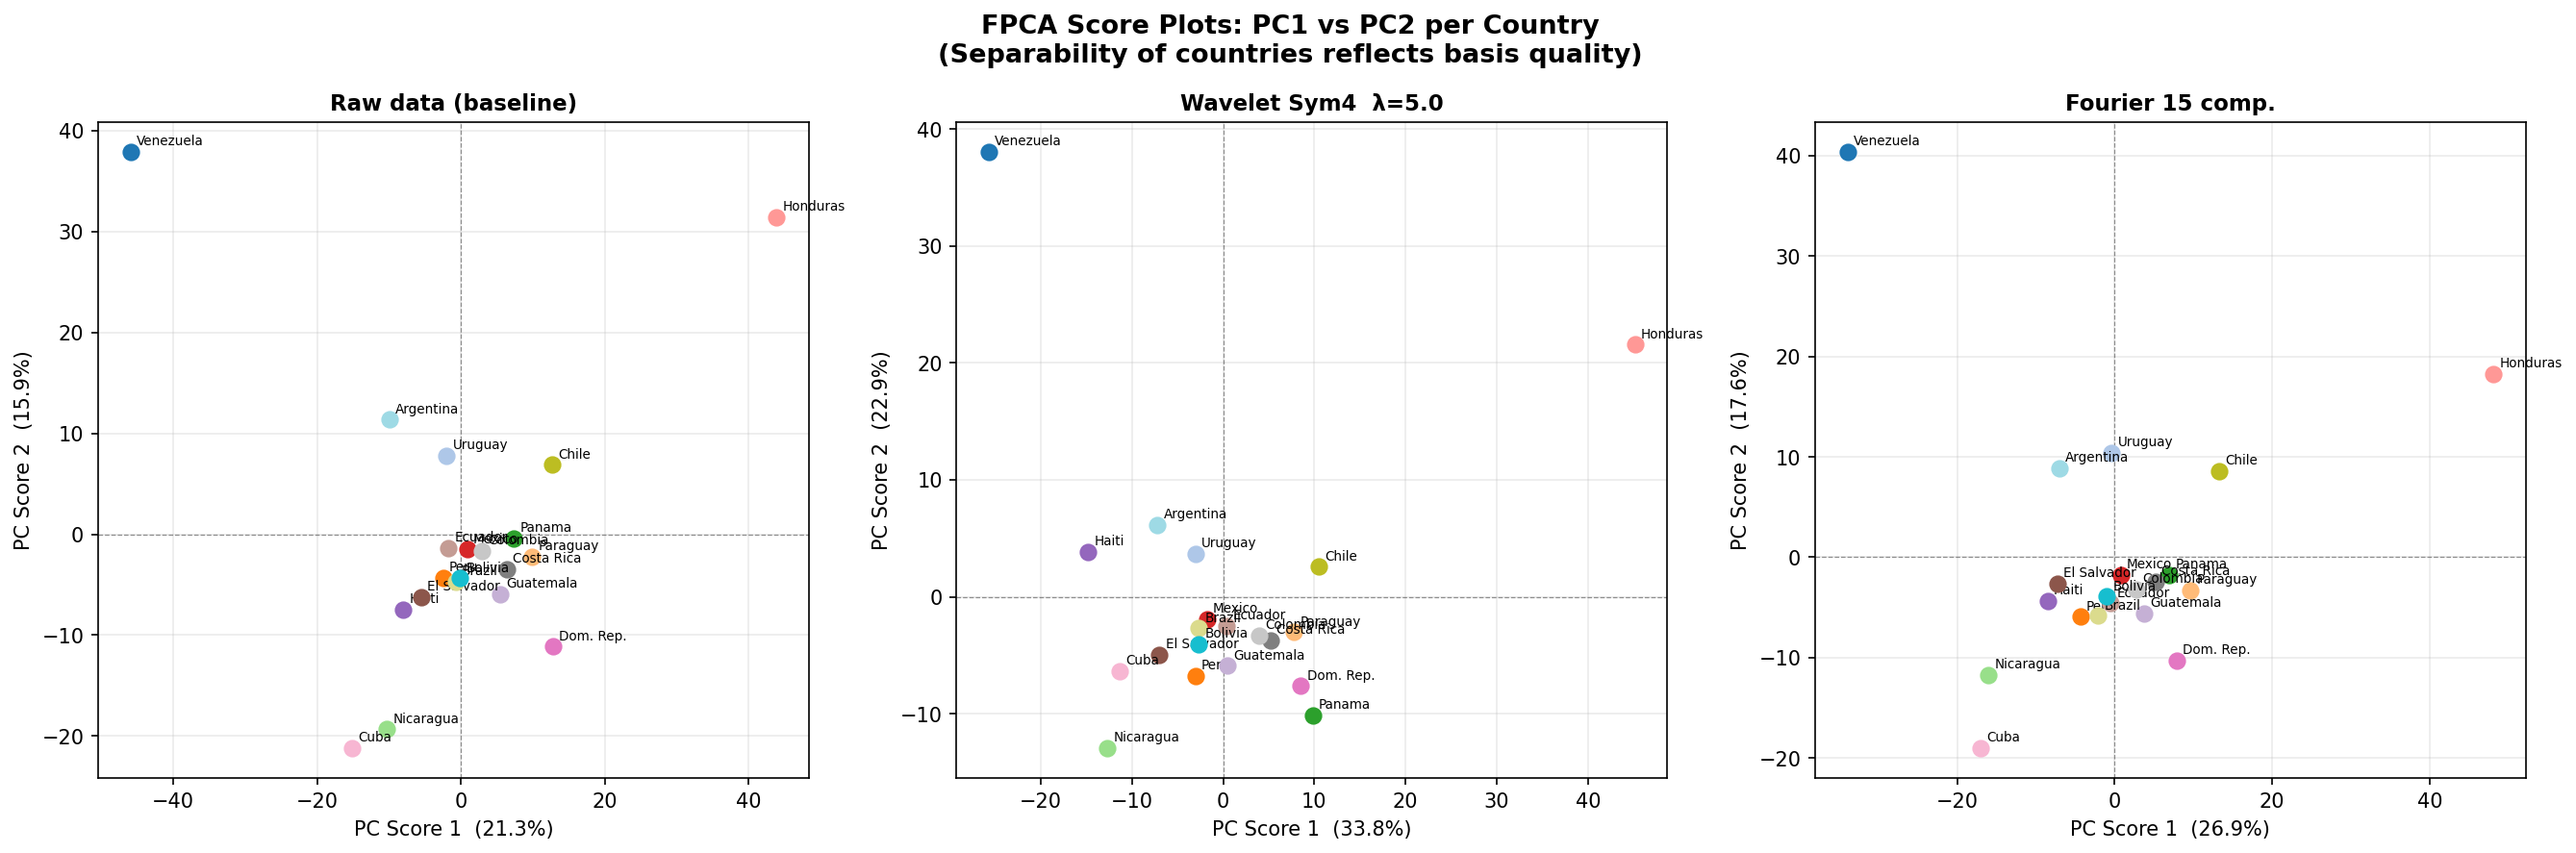
\includegraphics[width=\textwidth]{figures/fig17_fpca_score_plots.png}
  \caption{Score plots (replicating Fig 8 of paper).}
  \label{fig:score_plots}
\end{figure}

The FPCA score plots (Figure~\ref{fig:score_plots}) project each country onto
the first two principal components. Three configurations are compared: raw data,
Wavelet Sym4 $\lambda = 5$, and Fourier $K = 15$.

Venezuela is consistently the most extreme outlier in the PC1 direction across
all three configurations, reflecting the unprecedented magnitude of its
post-2015 economic contraction. Honduras is consistently separated in the PC2
direction, driven by its anomalous high-growth period in the 1990s.

Under the Wavelet Sym4 representation, the stable Central American economies
(Guatemala, El Salvador, Costa Rica) cluster more tightly than under the raw
data representation, suggesting that wavelet thresholding selectively removes
idiosyncratic noise while preserving systematic regional co-movement. This
improved cluster structure has direct implications for downstream applications
such as functional hierarchical clustering or regional policy grouping.

\subsection{Wavelet Energy Distribution}
\label{subsec:energy}

Figure~\ref{fig:energy} shows the distribution of wavelet energy across
decomposition levels A4 (coarsest approximation), D4, D3, D2, and D1 (finest
detail) for Venezuela, Colombia, and Argentina under the three wavelet families
tested.

\begin{figure}[H]
  \centering
  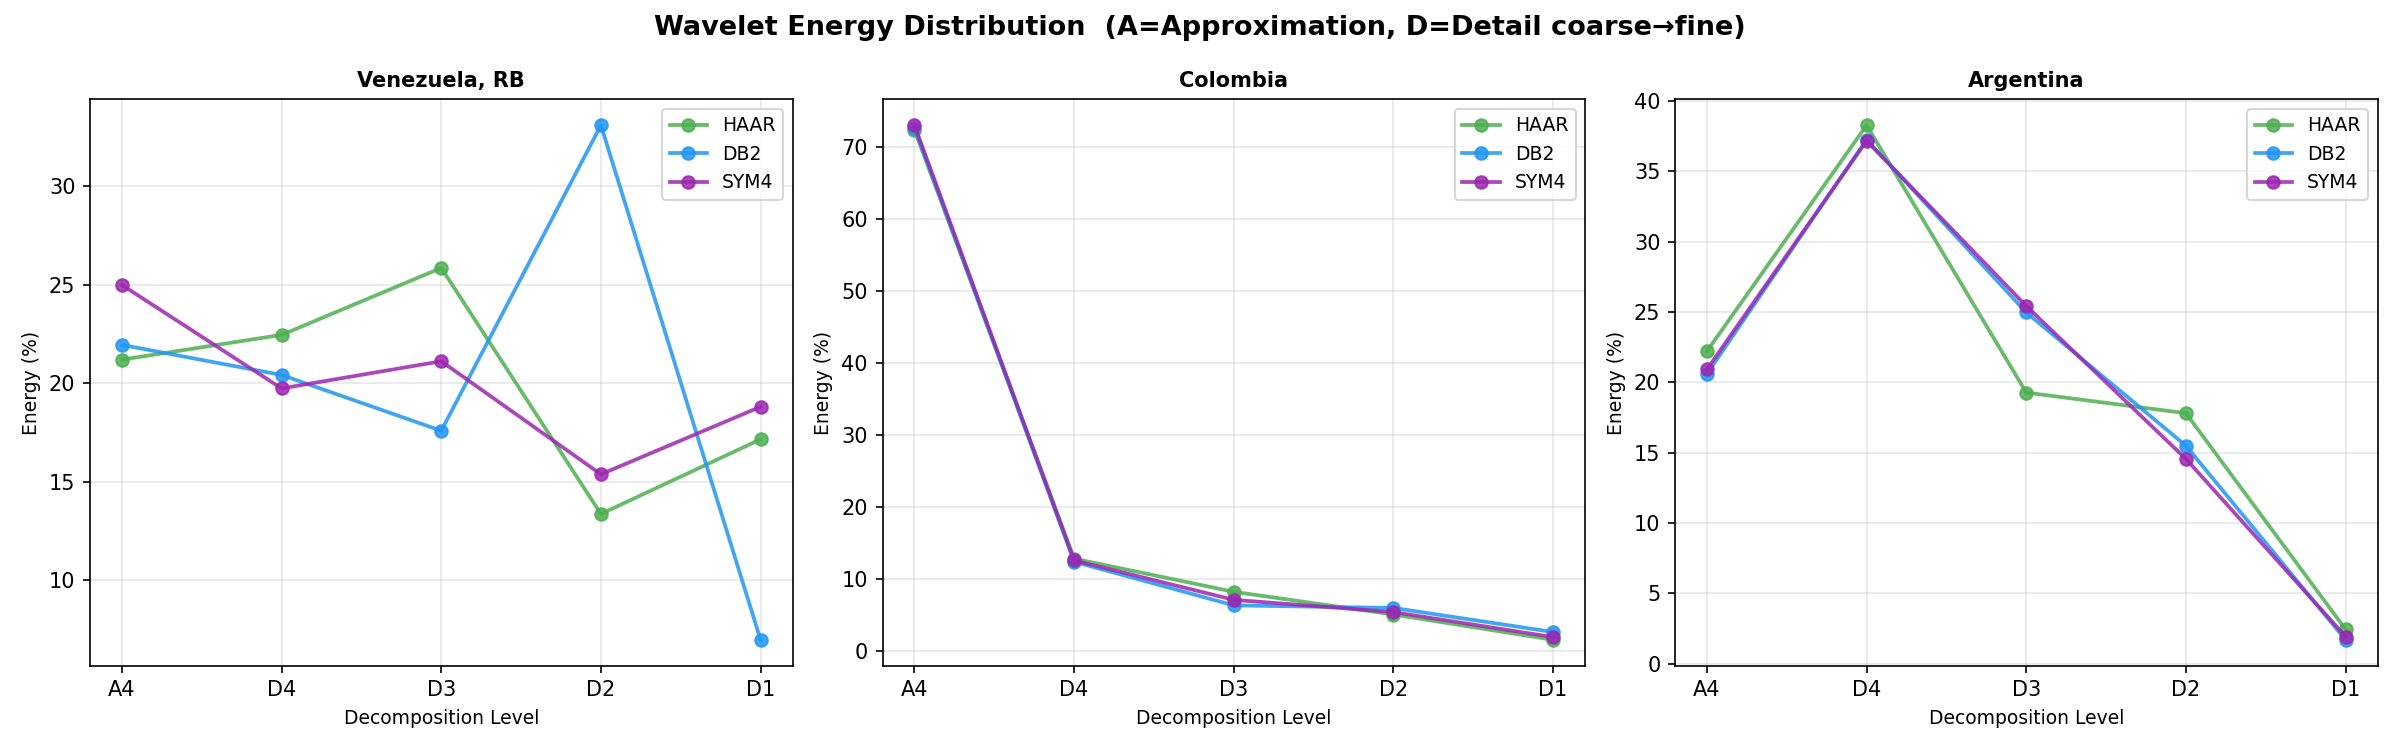
\includegraphics[width=\textwidth]{figures/fig09b_energy_distribution.png}
  \caption{Sparsity at matched RMSE — all 20 countries.}
  \label{fig:energy}
\end{figure}

Colombia concentrates approximately 72\% of its wavelet energy in the A4
approximation component: its GDP trajectory is dominated by a smooth long-run
trend with negligible fine-scale variation. These economies are well-approximated
by Sobolev-class functions, for which B-splines are theoretically optimal.

Venezuela distributes energy relatively evenly across all decomposition levels.
No single scale dominates, confirming that its growth process has genuine
multiscale structure that cannot be captured by any single-scale basis.
Argentina concentrates its energy primarily in the D4 level (the coarsest detail,
corresponding to fluctuations at time scales of 8--16 years), consistent with
Argentina's well-documented boom-bust cycle operating at medium-term horizons.

These country-specific energy profiles are economically interpretable and would
be entirely invisible to a global basis such as B-splines or Fourier series. The
wavelet multiresolution decomposition provides a natural language for identifying
\emph{at which time scales} each country's growth variation operates---an
original analytical contribution relative to \cite{padilla2020}.

\section{Summary of Findings}
\label{sec:summary}

The empirical results, taken together, support the following conclusions.

The \textbf{B-spline basis} achieves low RMSE through over-smoothing. It discards
economically significant crisis episodes as noise and produces FPCA results that
conflate trend removal with variance organisation. Its apparent parsimony is an
artefact of the smoothing constraint, not evidence of an efficient functional
representation.

The \textbf{Fourier basis} is inappropriate for this dataset because GDP growth
rates exhibit no dominant periodic structure (confirmed by power spectral
analysis) and contain localised structural breaks that produce Gibbs-type
artefacts under finite-term Fourier approximation.

The \textbf{wavelet basis}, at moderate thresholding, provides the most
informative functional representation across all metrics examined: it preserves
crisis episodes via sparse representation of localised shocks, reveals
country-specific multiscale variance structure through energy distribution
analysis, produces economically interpretable FPCA modes, and offers a principled
tradeoff between smoothness and fidelity via the threshold parameter $\lambda$.
These advantages are most pronounced for the highly volatile economies---Venezuela,
Nicaragua, Argentina, Honduras---where the gap between B-spline and wavelet
representation is largest.

The finding does not support the simple claim that wavelets outperform B-splines
on a scalar RMSE metric. Rather, it supports the more nuanced and more useful
conclusion that \emph{the choice of functional basis determines what the analyst
sees in the data}, and that for volatile, multiscale economic series, the wavelet
basis provides a fundamentally richer and more economically meaningful
representation than the alternatives tested here.